%% FEUP THESIS STYLE for LaTeX2e
%% how to use feupteses (English version)
%%
%% FEUP, JCL & JCF, 31 July 2012
%%
%% PLEASE send improvements to jlopes at fe.up.pt and to jcf at fe.up.pt
%%

%%========================================
%% Commands: pdflatex tese
%%           bibtex tese
%%           makeindex tese (only if creating an index) 
%%           pdflatex tese
%% Alternative:
%%          latexmk -pdf tese.tex
%%========================================

\documentclass[11pt,a4paper,twoside,openright]{report}

%% For iso-8859-1 (latin1), comment next line and uncomment the second line
\usepackage[utf8]{inputenc}
%\usepackage[latin1]{inputenc}

%% English version

%% MIEIC options
\usepackage[mieic]{feupteses}
%\usepackage[mieic,juri]{feupteses}
%\usepackage[mieic,final]{feupteses}
%\usepackage[mieic,final,onpaper]{feupteses}

%% Additional options for feupteses.sty: 
%% - onpaper: links are not shown (for paper versions)
%% - backrefs: include back references from bibliography to citation place

%% Uncomment the next lines if side by side graphics used
%\usepackage[lofdepth,lotdepth]{subfig}
%\usepackage{graphicx}
%\usepackage{float}

%% Include color package
\usepackage{color}
\definecolor{cloudwhite}{cmyk}{0,0,0,0.025}

%% Include source-code listings package
\usepackage{listings}
\lstset{ %
 language=C,                        % choose the language of the code
 basicstyle=\footnotesize\ttfamily,
 keywordstyle=\bfseries,
 numbers=left,                      % where to put the line-numbers
 numberstyle=\scriptsize\texttt,    % the size of the fonts that are used for the line-numbers
 stepnumber=1,                      % the step between two line-numbers. If it's 1 each line will be numbered
 numbersep=8pt,                     % how far the line-numbers are from the code
 frame=tb,
 float=htb,
 aboveskip=8mm,
 belowskip=4mm,
 backgroundcolor=\color{cloudwhite},
 showspaces=false,                  % show spaces adding particular underscores
 showstringspaces=false,            % underline spaces within strings
 showtabs=false,                    % show tabs within strings adding particular underscores
 tabsize=2,	                    % sets default tabsize to 2 spaces
 captionpos=b,                      % sets the caption-position to bottom
 breaklines=true,                   % sets automatic line breaking
 breakatwhitespace=false,           % sets if automatic breaks should only happen at whitespace
 escapeinside={\%*}{*)},            % if you want to add a comment within your code
 morekeywords={*,var,template,new}  % if you want to add more keywords to the set
}

%% Uncomment to create an index (at the end of the document)
%\makeindex

%% Path to the figures directory
%% TIP: use folder ``figures'' to keep all your figures
\graphicspath{{figures/}}

%%----------------------------------------
%% TIP: if you want to define more macros, use an external file to keep them
%!TEX root = ../mieic.tex

%some macro definitions

% format
\newcommand{\class}[1]{{\normalfont\slshape #1\/}}

% entities
\newcommand{\Feup}{Faculdade de Engenharia da Universidade do Porto}

\newcommand{\svg}{\class{SVG}}
\newcommand{\scada}{\class{SCADA}}
\newcommand{\scadadms}{\class{SCADA/DMS}}

%%----------------------------------------

%%========================================
%% Start of document
%%========================================
\begin{document}

%%----------------------------------------
%% Information about the work
%%----------------------------------------
\title{Title of the Dissertation}
\author{Name of the Author}

%% Uncomment next line for date of submission
%\thesisdate{July 31, 2008}

%%Uncomment next line for copyright text if used
%\copyrightnotice{Name of the Author, 2008}

\supervisor{Supervisor}{Name of the Supervisor}

%% Uncomment next line if necessary
%\supervisor{Second Supervisor}{Name of the Supervisor}

%% Uncomment committee stuff in the final version if used
%\committeetext{Approved in oral examination by the committee:}
%\committeemember{Chair}{Doctor Name of the President}
%\committeemember{External Examiner}{Doctor Name of the Examiner}
%\committeemember{Supervisor}{Doctor Name of the Supervisor}
%\signature

%% Specify cover logo (in folder ``figures'')
\logo{uporto-feup.pdf}

%% Uncomment next line for additional text  below the author's name (front page)
%\additionalfronttext{Preparação da Dissertação}

%%----------------------------------------
%% Preliminary materials
%%----------------------------------------

% remove unnecssary \include{} commands
\begin{Prolog}
  \chapter*{Abstract}

Here goes the abstract written in English.

Lorem ipsum dolor sit amet, consectetuer adipiscing elit. Sed vehicula
lorem commodo dui. Fusce mollis feugiat elit. Cum sociis natoque
penatibus et magnis dis parturient montes, nascetur ridiculus
mus. Donec eu quam. Aenean consectetuer odio quis nisi. Fusce molestie
metus sed neque. Praesent nulla. Donec quis urna. Pellentesque
hendrerit vulputate nunc. Donec id eros et leo ullamcorper
placerat. Curabitur aliquam tellus et diam. 

Ut tortor. Morbi eget elit. Maecenas nec risus. Sed ultricies. Sed
scelerisque libero faucibus sem. Nullam molestie leo quis
tellus. Donec ipsum. Nulla lobortis purus pharetra turpis. Nulla
laoreet, arcu nec hendrerit vulputate, tortor elit eleifend turpis, et
aliquam leo metus in dolor. Praesent sed nulla. Mauris ac augue. Cras
ac orci. Etiam sed urna eget nulla sodales venenatis. Donec faucibus
ante eget dui. Nam magna. Suspendisse sollicitudin est et mi. 

Fusce sed ipsum vel velit imperdiet dictum. Sed nisi purus, dapibus
ut, iaculis ac, placerat id, purus. Integer aliquet elementum
libero. Phasellus facilisis leo eget elit. Nullam nisi magna, ornare
at, aliquet et, porta id, odio. Sed volutpat tellus consectetuer
ligula. Phasellus turpis augue, malesuada et, placerat fringilla,
ornare nec, eros. Class aptent taciti sociosqu ad litora torquent per
conubia nostra, per inceptos himenaeos. Vivamus ornare quam nec sem
mattis vulputate. Nullam porta, diam nec porta mollis, orci leo
condimentum sapien, quis venenatis mi dolor a metus. Nullam
mollis. Aenean metus massa, pellentesque sit amet, sagittis eget,
tincidunt in, arcu. Vestibulum porta laoreet tortor. Nullam mollis
elit nec justo. In nulla ligula, pellentesque sit amet, consequat sed,
faucibus id, velit. Fusce purus. Quisque sagittis urna at quam. Ut eu
lacus. Maecenas tortor nibh, ultricies nec, vestibulum varius, egestas
id, sapien. 

Phasellus ullamcorper justo id risus. Nunc in leo. Mauris auctor
lectus vitae est lacinia egestas. Nulla faucibus erat sit amet lectus
varius semper. Praesent ultrices vehicula orci. Nam at metus. Aenean
eget lorem nec purus feugiat molestie. Phasellus fringilla nulla ac
risus. Aliquam elementum aliquam velit. Aenean nunc odio, lobortis id,
dictum et, rutrum ac, ipsum. 

Ut tortor. Morbi eget elit. Maecenas nec risus. Sed ultricies. Sed
scelerisque libero faucibus sem. Nullam molestie leo quis
tellus. Donec ipsum. Nulla lobortis purus pharetra turpis. Nulla
laoreet, arcu nec hendrerit vulputate, tortor elit eleifend turpis, et
aliquam leo metus in dolor. Praesent sed nulla. Mauris ac augue. Cras
ac orci. Etiam sed urna eget nulla sodales venenatis. Donec faucibus
ante eget dui. Nam magna. Suspendisse sollicitudin est et mi. 

Phasellus ullamcorper justo id risus. Nunc in leo. Mauris auctor
lectus vitae est lacinia egestas. Nulla faucibus erat sit amet lectus
varius semper. Praesent ultrices vehicula orci. Nam at metus. Aenean
eget lorem nec purus feugiat molestie. Phasellus fringilla nulla ac
risus. Aliquam elementum aliquam velit. Aenean nunc odio, lobortis id,
dictum et, rutrum ac, ipsum. 

Ut tortor. Morbi eget elit. Maecenas nec risus. Sed ultricies. Sed
scelerisque libero faucibus sem. Nullam molestie leo quis
tellus. Donec ipsum. 

\chapter*{Resumo}

O Resumo fornece ao leitor um sumário do conteúdo da dissertação.
Deverá ser breve mas conter detalhe suficiente e, uma vez que é a porta
de entrada para a dissertação, deverá dar ao leitor uma boa impressão
inicial.

Este texto inicial da dissertação é escrito no fim e resume numa
página, sem referências externas, o tema e o contexto do trabalho, a
motivação e os objectivos, as metodologias e técnicas empregues, os
principais resultados alcançados e as conclusões.

Este documento ilustra o formato a usar em dissertações na \Feup.
São dados exemplos de margens, cabeçalhos, títulos, paginação, estilos
de índices, etc. 
São ainda dados exemplos de formatação de citações, figuras e tabelas,
equações, referências cruzadas, lista de referências e índices.
%Este documento não pretende exemplificar conteúdos a usar. 
É usado texto descartável, \emph{Loren Ipsum}, para preencher a
dissertação por forma a ilustrar os formatos.

Seguem-se umas notas breves mas muito importantes sobre a versão 
provisória e a versão final do documento. 
A versão provisória, depois de verificada pelo orientador e de 
corrigida em contexto pelo autor, deve ser publicada na página 
pessoal de cada estudante/dissertação, juntamente com os dois 
resumos, em português e em inglês; deve manter a marca da água, 
assim como a numeração de linhas conforme aqui se demonstra.

A versão definitiva, a produzir somente após a defesa, em versão 
impressa (dois exemplares com capas próprias FEUP) e em versão 
eletrónica (6 CDs com "rodela" própria FEUP), deve ser limpa da marca de 
água e da numeração de linhas e deve conter a identificação, na primeira 
página, dos elementos do júri respetivo. 
Deve ainda, se for o caso, ser corrigida de acordo com as instruções 
recebidas dos elementos júri.

Lorem ipsum dolor sit amet, consectetuer adipiscing elit. Sed vehicula
lorem commodo dui. Fusce mollis feugiat elit. Cum sociis natoque
penatibus et magnis dis parturient montes, nascetur ridiculus
mus. Donec eu quam. Aenean consectetuer odio quis nisi. Fusce molestie
metus sed neque. Praesent nulla. Donec quis urna. Pellentesque
hendrerit vulputate nunc. Donec id eros et leo ullamcorper
placerat. Curabitur aliquam tellus et diam. 

Ut tortor. Morbi eget elit. Maecenas nec risus. Sed ultricies. Sed
scelerisque libero faucibus sem. Nullam molestie leo quis
tellus. Donec ipsum. Nulla lobortis purus pharetra turpis. Nulla
laoreet, arcu nec hendrerit vulputate, tortor elit eleifend turpis, et
aliquam leo metus in dolor. Praesent sed nulla. Mauris ac augue. Cras
ac orci. Etiam sed urna eget nulla sodales venenatis. Donec faucibus
ante eget dui. Nam magna. Suspendisse sollicitudin est et mi. 

Phasellus ullamcorper justo id risus. Nunc in leo. Mauris auctor
lectus vitae est lacinia egestas. Nulla faucibus erat sit amet lectus
varius semper. Praesent ultrices vehicula orci. Nam at metus. Aenean
eget lorem nec purus feugiat molestie. Phasellus fringilla nulla ac
risus. Aliquam elementum aliquam velit. Aenean nunc odio, lobortis id,
dictum et, rutrum ac, ipsum. 

Ut tortor. Morbi eget elit. Maecenas nec risus. Sed ultricies. Sed
scelerisque libero faucibus sem. Nullam molestie leo quis
tellus. Donec ipsum. 
 % the abstract
  \chapter*{Acknowledgements}

Aliquam id dui. Nulla facilisi. Nullam ligula nunc, viverra a, iaculis
at, faucibus quis, sapien. Cum sociis natoque penatibus et magnis dis
parturient montes, nascetur ridiculus mus. Curabitur magna ligula,
ornare luctus, aliquam non, aliquet at, tortor. Donec iaculis nulla
sed eros. Sed felis. Nam lobortis libero. Pellentesque
odio. Suspendisse potenti. Morbi imperdiet rhoncus magna. Morbi
vestibulum interdum turpis. Pellentesque varius. Morbi nulla urna,
euismod in, molestie ac, placerat in, orci. 

Ut convallis. Suspendisse luctus pharetra sem. Sed sit amet mi in diam
luctus suscipit. Nulla facilisi. Integer commodo, turpis et semper
auctor, nisl ligula vestibulum erat, sed tempor lacus nibh at
turpis. Quisque vestibulum pulvinar justo. Class aptent taciti
sociosqu ad litora torquent per conubia nostra, per inceptos
himenaeos. Nam sed tellus vel tortor hendrerit pulvinar. Phasellus
eleifend, augue at mattis tincidunt, lorem lorem sodales arcu, id
volutpat risus est id neque. Phasellus egestas ante. Nam porttitor
justo sit amet urna. Suspendisse ligula nunc, mollis ac, elementum
non, venenatis ut, mauris. Mauris augue risus, tempus scelerisque,
rutrum quis, hendrerit at, nunc. Nulla posuere porta orci. Nulla dui. 

Fusce gravida placerat sem. Aenean ipsum diam, pharetra vitae, ornare
et, semper sit amet, nibh. Nam id tellus. Etiam ultrices. Praesent
gravida. Aliquam nec sapien. Morbi sagittis vulputate dolor. Donec
sapien lorem, laoreet egestas, pellentesque euismod, porta at,
sapien. Integer vitae lacus id dui convallis blandit. Mauris non
sem. Integer in velit eget lorem scelerisque vehicula. Etiam tincidunt
turpis ac nunc. Pellentesque a justo. Mauris faucibus quam id
eros. Cras pharetra. Fusce rutrum vulputate lorem. Cras pretium magna
in nisl. Integer ornare dui non pede. 

\vspace{10mm}
\flushleft{The Name of the Author}
  % the acknowledgments
  \cleardoublepage
\thispagestyle{plain}

\vspace*{8cm}

\begin{flushright}
   \textsl{``You should be glad that bridge fell down. \\
           I was planning to build thirteen more to that same design''} \\
\vspace*{1.5cm}
           Isambard Kingdom Brunel
\end{flushright}
       % initial quotation if desired
  \cleardoublepage
  \pdfbookmark[0]{Table of Contents}{contents}
  \tableofcontents
  \cleardoublepage
  \pdfbookmark[0]{List of Figures}{figures}
  \listoffigures
  \cleardoublepage
  \pdfbookmark[0]{List of Tables}{tables}
  \listoftables
  \chapter*{Abbreviations}
\chaptermark{ABBREVIATIONS}

\begin{flushleft}
\begin{tabular}{l p{0.8\linewidth}}
ADT      & Abstract Data Type\\
ANDF     & Architecture-Neutral Distribution Format\\
API      & Application Programming Interface\\
CAD      & Computer-Aided Design\\
CASE     & Computer-Aided Software Engineering\\
CORBA    & Common Object Request Broker Architecture\\
UNCOL    & UNiversal COmpiler-oriented Language\\
Loren    & Lorem ipsum dolor sit amet, consectetuer adipiscing
elit. Sed vehicula lorem commodo dui\\
WWW      & \emph{World Wide Web}
\end{tabular}
\end{flushleft}

  % the list of abbreviations used
\end{Prolog}

%%----------------------------------------
%% Body
%%----------------------------------------
\StartBody

%% TIP: use a separate file for each chapter
%!TEX root = ../mieic.tex

\chapter{Introdução} \label{chap:intro}



\section{Contexto/Enquadramento} \label{sec:context}

Bem longe vão os tempos, antes da Internet, em que ouvir e descobrir música nova era um desafio por si só.
Agora, com alguns cliques, temos acesso a um catálogo de música tão grande, que o nosso cérebro não consegue processar.

Existem dezenas de serviços online que oferecem isso mesmo.
Alguns especializam-se na criação/geração de playlists (que funcionam como rádios), outros em expandir o catálogo de música e outros focam-se mais na sugestão e recomendação de artistas/álbuns/músicas personalizada para os utilizadores.
Estes últimos, apresentam as sugestões de conteúdo ao utilizador de uma forma rudimentar como listas ou em grelha.

No entanto, listas ou grelhas não fornecem ao utilizador qualquer tipo de informação adicional sobre a relação entre os artistas nem justificam a sua semelhança \cite{Lamere2008}.
Até fazem parecer que não existe nenhuma relação/ligação entre os artistas recomendados, o que não é verdade.

Essas relações existem e podem ser representadas como uma rede de artistas interligados num grafo, onde cada nó é um artista de música, e cada ligação entre nós representa uma ligação forte de parecença entre os artistas.
Este é o conceito que o RAMA\footnote{http://rama.inescporto.pt}, projeto desenvolvido no INESC Porto\footnote{http://inescporto.pt}, usa. \cite{Costa2008} \cite{Sarmento2009} \cite{Costa2009} \cite{Gouyon2011}

\section{Motivação e Objetivos} \label{sec:goals}


A partir de uma pesquisa de um artista de música, o RAMA cria e desenha um grafo que ajuda o utilizador a explorar música que lhe possa interessar de uma forma muito mais natural e informativa.
A informação que o RAMA usa é retirada do serviço Last.fm\footnote{http://last.fm}.

No entanto, quando um utilizador pretende ouvir uma música de um artista, é usado stream do Youtube\footnote{http://youtube.com}. 
Apesar de este oferecer um catálogo alargado de música, o mesmo não é indicado para esta funcionalidade pois não fornece nenhum tipo de API\footnote{Application Programming Interface} orientada a música, nem a qualidade de som do stream é adequada.

Por forma a resolver este problema, foram analisadas várias possibilidades de integrar um serviço de streaming de música no RAMA, ou vice-versa.
A escolha final foi desenvolver uma aplicação (como plugin) para o Spotify\footnote{http://spotify.com}.
Desta forma, os utilizadores Spotify poderão ter uma experiência mais natural e integrada, usufruindo de todas as funcionalidades que o RAMA oferece, dentro do Spotify.


O objetivo final do projeto é poder oferecer aos utilizadores do Spotify, uma experiência de descoberta de música muito mais agradável, natural e detalhada.
No entanto, para avaliar e validar o resultado final, será necessário fazer testes com utilizadores finais para comparar a sua experiência no Spotify com e sem a aplicação desenvolvida.

Desta forma, o desenvolvimento da aplicação será feito de forma iterativa, implementando as funcionalidades que o RAMA oferece, e quando esta estiver ao nível do RAMA, serão realizados testes cuidados com os utilizadores à medida que se melhora a implementação com o seu feedback.
 \\
 \\
Em suma, os objetivos deste projeto são:

\begin{itemize}
  \item Melhorar a forma de apresentação da recomendação de conteúdo dentro do Spotify;
  \item Dar mais poder ao utilizador na descoberta de música nova;
  \item Tornar a experiência de descoberta mais interessante e cativante.
\end{itemize}

\section{Projeto} \label{sec:proj}

A aplicação a desenvolver será uma alternativa ao modo de descoberta do Spotify.
No momento de escrita deste relatório, o modo de descoberta/recomendação de música do Spotify, comparativamente ao do Last.fm, é simples: apresenta recomendaçõs em forma de grelha.



\section*{}
\emph{
Na continuação da secção anterior, e apenas no caso de ser um Projeto
e não uma Dissertação, esta secção apresenta resumidamente o projeto.}


\section{Estrutura da Dissertação} \label{sec:struct}

\emph{Para além da introdução, esta dissertação contém mais x capítulos.
No capítulo~\ref{chap:sota}, é descrito o estado da arte e são
apresentados trabalhos relacionados.
%\todoline{Complete the document structure.}
No capítulo~\ref{chap:chap3}, é explicado em detalhe em que consiste o projeto
No capítulo~\ref{chap:chap4} praesent sit amet sem. 
No capítulo~\ref{chap:concl}  posuere, ante non tristique
consectetuer, dui elit scelerisque augue, eu vehicula nibh nisi ac
est. 
} 
%!TEX root = ../mieic.tex

\chapter{State of The Art} \label{chap:chap2}

\section*{}

\section{Introduction}

In this chapter, the most relevant web services for this thesis will be analysed.

The proposed methodology focus on how the content is presented and less on what the content is (without discarding its importance).
Even so, some projects that focus on the content will be analysed.

The presented projects often use external data bases (like last.fm) to fetch metadata from.
This is the preferred way, since those are the most complete sets of information. 

\section{Related and Similar Services} % (fold)
\label{sec:projetos_relacionados}

\subsection{Liveplasma - liveplasma.com} % (fold)
\label{sub:liveplasma}

liveplasma.com is a \emph{flash}\footnote{http://get.adobe.com/flashplayer} application that not only it allows to see a graph of music artists, but also of books and movies.

The interaction with the graph is very faulted: no changes to the graph are allowed, and the user can easily make a mistake and perform unwanted actions like redrawing the graph with another artist as the root node.

\begin{figure}
  \begin{center}
    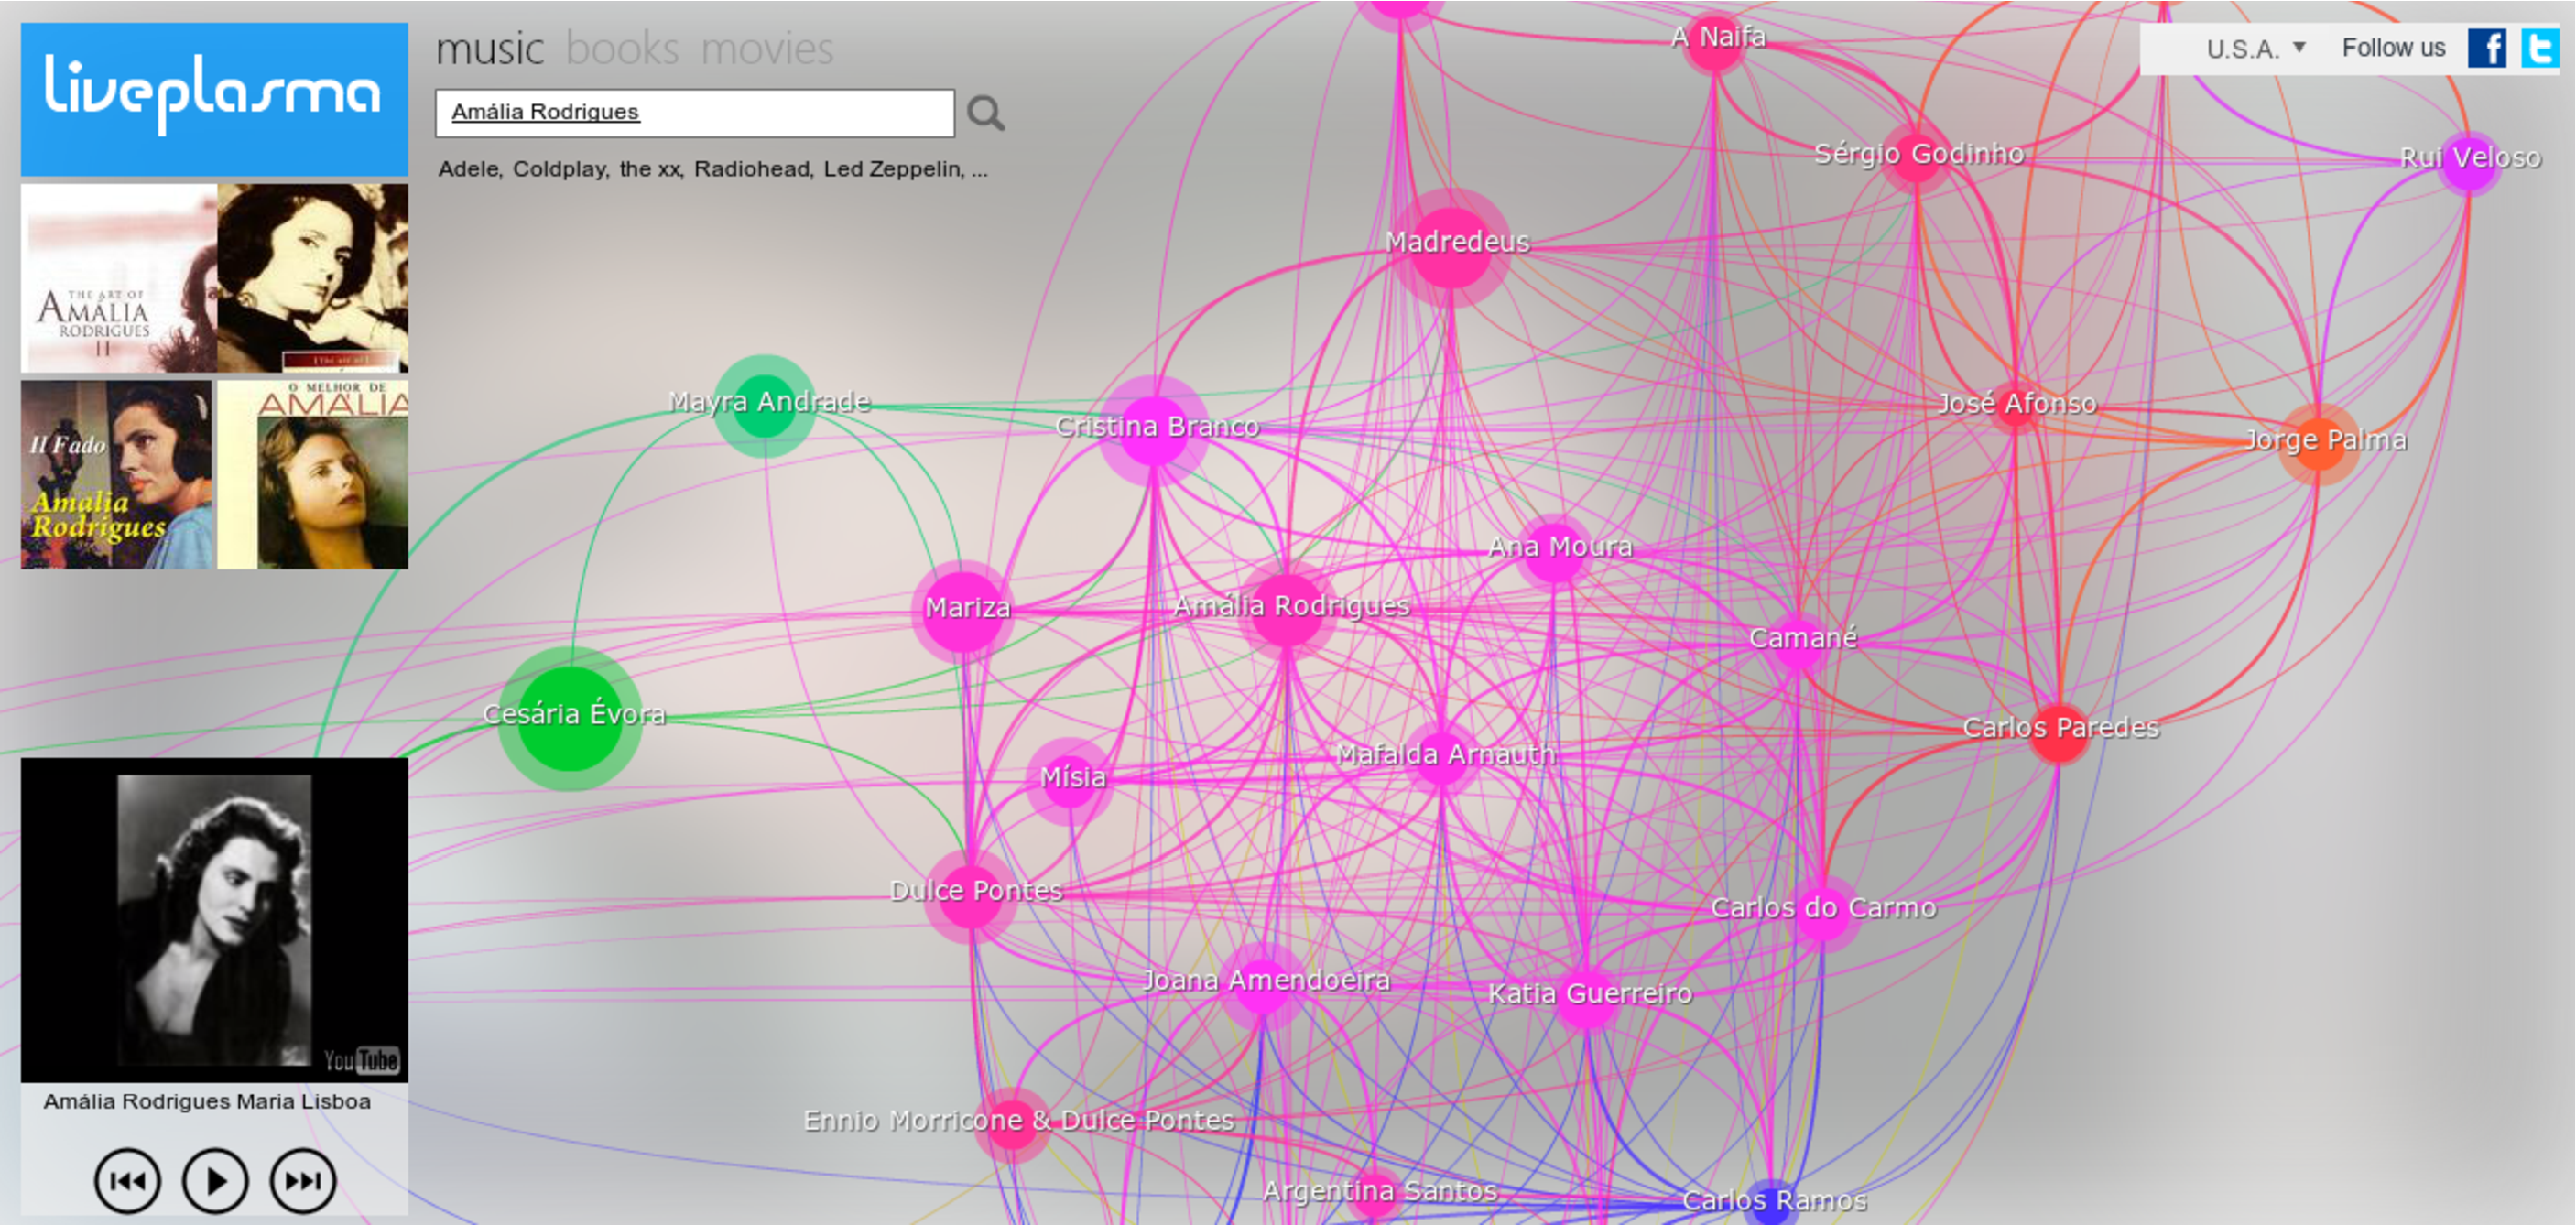
\includegraphics[width=\textwidth]{liveplasma.pdf}
  \end{center}
  \caption{liveplasma: search result for "Amália Rodrigues"; upper left corner: artist albums; lower left corner: youtube's \emph{mini-player}}
  \label{fig:sota_liveplasma}
\end{figure}

Na figura \ref{fig:sota_liveplasma} podemos ver o resultado de uma pesquisa.
É possível ver a grelha com os álbums que o artista lançou, que redirecionam o utilizador para a Amazon\footnote{http://amazon.com} para comprar os álbums e um \emph{mini-player} que começa a reproduzir uma música do artista diretamente do Youtube.

É possível controlar que músicas são reproduzidas de uma forma interessante: ao passar o rato por cima de um nó, aparece dois botões que permitem reproduzir música só do próprio artista (botão \emph{only}) ou só de artistas parecidos (botão \emph{similar}).
É possível ver esses botões na figura \ref{fig:sota_liveplasma2}

\begin{figure}[tb]
  \begin{center}
    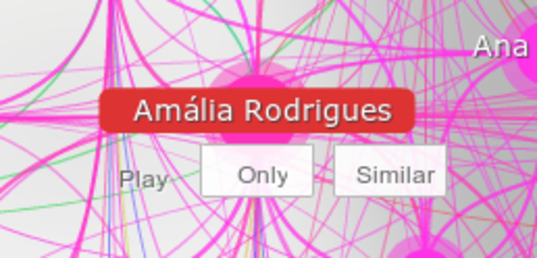
\includegraphics[]{liveplasma2.pdf}
  \end{center}
  \caption{liveplasma: interface para reprodução de música. Botão \emph{similar} reproduz músicas de artistas parecidos; Botão \emph{only} só reproduz músicas do artista pesquisado.}
  \label{fig:sota_liveplasma2}
\end{figure}

\subsubsection{Prós} % (fold)
\label{ssub:liveplasma_pros}

Os aspetos interessantes desta ferramenta são:

\begin{itemize}
  \item Links para compra dos álbums
  \item Reproduzir músicas de artistas semelhantes
\end{itemize}

% subsubsection pros (end)

\subsubsection{Contras} % (fold)
\label{ssub:liveplasma_contras}

O grafo desenhado é bastante confuso quando existem muitos nós com muitas ligações.
Isto acontece quando existem muitos artistas semelhantes.
Para além disso, são atribuídas cores aos nós que devem identificar o grau de parecença entre os artistas.
No entanto não existe nenhum tipo de informação que explique qual o seu verdadeiro significado ao utilizador, assim como também não existe uma explicação das ligações entre os nós.

É também de notar que o tamanho dos nós é diretamente proporcional à popularidade dos artistas respectivos, mas mais uma vez, este tipo de informação não é dada ao utilizador.

Outra falha a apontar é o facto de não se conseguir distinguir o nó de pesquisa dos restantes resultados em \ref{fig:sota_liveplasma} por exemplo.

% subsubsection contras (end)

\subsubsection{Resumo} % (fold)
\label{ssub:liveplasma_resumo}

Em suma, o liveplasma é usável, mas peca por ter muitas cores e ligações que tornam a experiência do utilizador ainda mais difícil do que a tradicional apresentação em lista ou grelha.

% subsubsection resumo (end)

% subsection liveplasma (end)

\subsection{Tuneglue - audiomap.tuneglue.net} % (fold)
\label{sub:tuneglue}

O Tuneglue é outro serviço do mesmo género (também desenvolvido em flash) que usa a base de dados do last.fm para recolher a informação dos artistas de música, assim como artistas relacionados.

Depois da pesquisa de um artista, por exemplo "Mariza", obtemos um grafo com apenas o nó de pesquisa. Ao clicar no nó é apresentado um menu com várias opções como se pode ver na figura \ref{fig:sota_tuneglue}.

\begin{figure}[tb]
  \begin{center}
    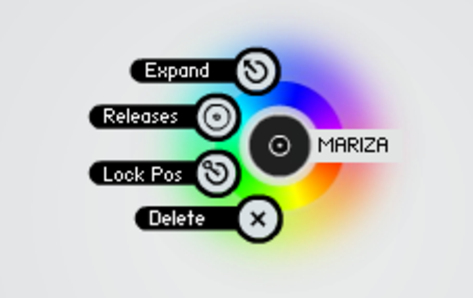
\includegraphics[]{tuneglue.pdf}
  \end{center}
  \caption{Tuneglue: menu que aparece ao clicar num nó.}
  \label{fig:sota_tuneglue}
\end{figure}

A partir deste menu é possível ver uma das principais diferenças que o Tuneglue tem em relação ao liveplasma (\ref{sub:liveplasma}): a edição do grafo.
É possível expandir, fixar e eliminar individualmente cada nó do grafo.
Ao expandir o nó inicial de pesquisa, os nós novos estão apenas e só diretamente relacionados com o nó pai, como se pode ver na figura~\ref{fig:sota_tuneglue2}.

\begin{figure}[tb]
  \begin{center}
    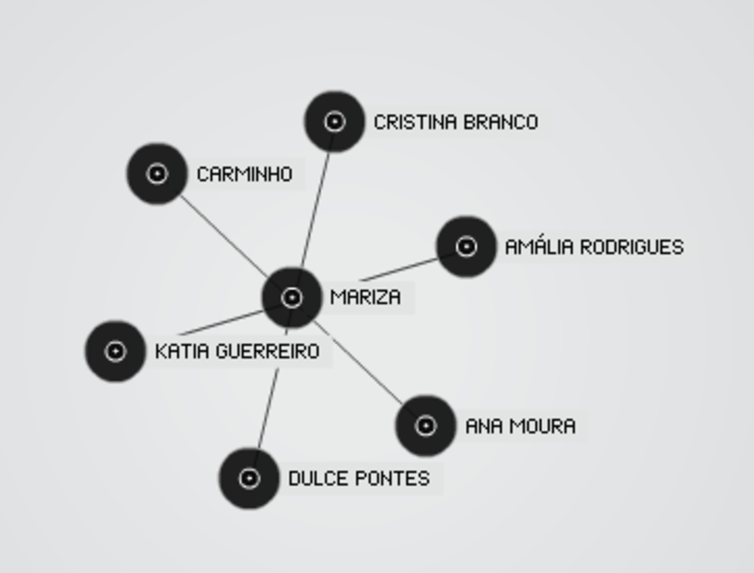
\includegraphics[]{tuneglue2.pdf}
  \end{center}
  \caption{Tuneglue: grafo depois do primeiro nó ser expandido.}
  \label{fig:sota_tuneglue2}
\end{figure}

Ao contrário do Liveplasma, o Tuneglue não faz uma pesquisa recursiva.

\subsubsection{Prós} % (fold)
\label{ssub:audiomap_pros}

Dá bastante liberdade ao utilizador, pois dá-lhe toda a responsabilidade na criação do grafo.
O utilizador sente que todo o grafo foi criação sua e dissimula o utilizador a pensar que foi este que descobriu novos artistas ao invés de receber recomendações.

% subsubsection pros (end)

\subsubsection{Contras} % (fold)
\label{ssub:audiomap_contras}

Mais uma vez, o facto da ferramenta ser feita em flash não ajuda a que a interface seja intuitiva.
Para além de pouco responsiva (o utilizador ao início pode-se sentir perdido por não saber o que fazer), é bastante uniforme, ou seja, não salienta diferenças entre cada artista, nem distingue as ligações entre eles.

% subsubsection contras (end)

\subsubsection{Resumo} % (fold)
\label{ssub:audiomap_resumo}

Em suma, o Tuneglue é inteligente por dar poder ao utilizador, mas ao mesmo tempo não existe um limite nesse poder.
E assim, é possível expandir o grafo até se tornar ilegível.



% subsubsection resumo (end)

% subsection tuneglue (end)

\subsection{MusicRoamer - musicroamer.com} % (fold)
\label{sub:musicroamer}

  O MusicRoamer é outra ferramenta que permite explorar música nova.
  Tal como o Tuneglue, este permitir construir o grafo à medida que se expande cada nó.



  \subsubsection{Prós} % (fold)
  \label{ssub:pros}

  
  Umas das funcionalidades interessantes do MusicRoamer são as várias opções de pesquisa (figura~\ref{fig:sota_musicroamer}):
  \begin{description}
    \item[Pesquisa por Artista] \hfill \\
      Tipo de pesquisa mais utilizada
    \item[Pesquisa por \emph{Keyword}] \hfill \\
      Usar palavras-chave como géneros musicais para pesquisar livremente
    \item[Pesquisa por perfil do Last.fm] \hfill \\
      Esta pesquisa gera um grafo para cada artista (os mais ouvidos pelo utilizador)
  \end{description}

  \begin{figure}[tb]
    \begin{center}
      
\includegraphics[width=\textwidth]{musicroamer.pdf}
    \end{center}
    \caption{MusicRoamer: Várias opções de pesquisa. Por artista; por \emph{keyword} e pelo perfil de utilizador do Last.fm}
    \label{fig:sota_musicroamer}
  \end{figure}

  Todas estas formas de pesquisa desenham um (ou mais) grafo(s) em que os nós são sempre artistas de música.

  O que esta ferramenta trás de novo é a forma como apresenta os grafos.
  A figura~\ref{fig:sota_musicroamer3} apresenta o resultado da pesquisa por Artista "Mariza".
  Imagens dos artistas são usadas para representar os nós, o que ajuda o utilizador a diferenciar os resultados.

  A ferramenta também disponibiliza alguns parâmetros de personalização do grafo (figura~\ref{fig:sota_musicroamer2}) como Zoom, Tamanho da repulsão, imagem entre os nós e o número de artistas de música que deve expandir de um nó.

  \begin{figure}[tb]
    \begin{center}
      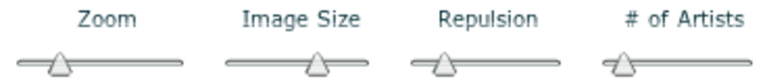
\includegraphics[width=\textwidth]{musicroamer2.pdf}
    \end{center}
    \caption{MusicRoamer: Parâmetros de personalização do grafo}
    \label{fig:sota_musicroamer2}
  \end{figure}



  \begin{figure}[tb]
    \begin{center}
      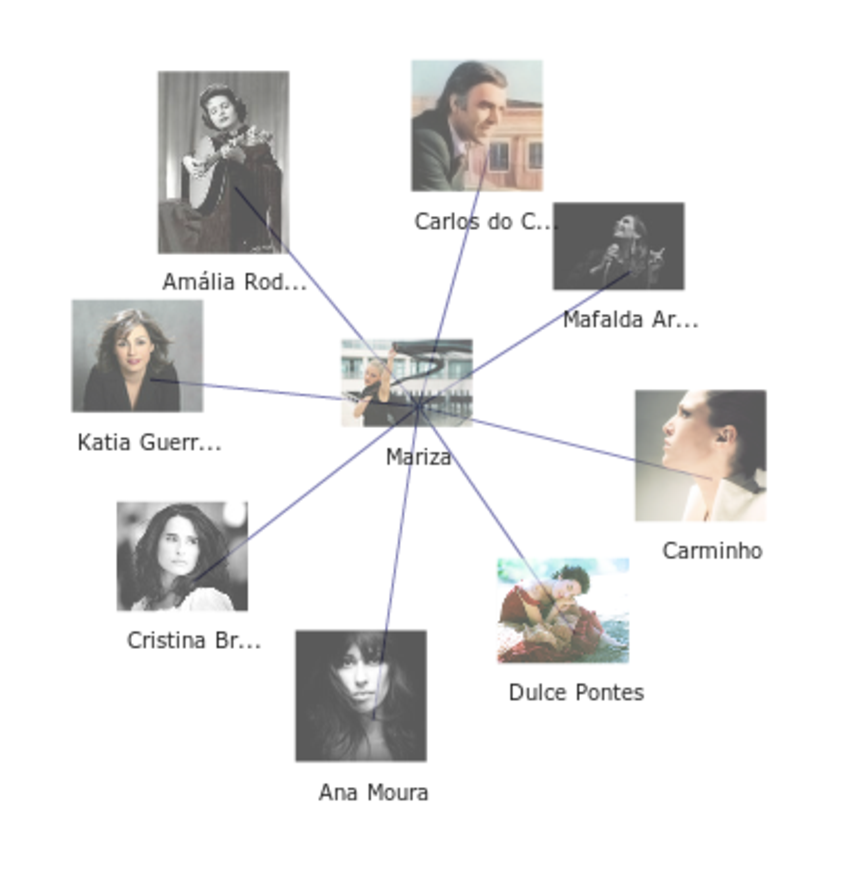
\includegraphics[width=\textwidth]{musicroamer3.pdf}
    \end{center}
    \caption{MusicRoamer: Representação visual do grafo de artistas}
    \label{fig:sota_musicroamer3}
  \end{figure}

  % subsubsection pros (end)

  \subsubsection{Contras} % (fold)
  \label{ssub:contras}

  Um problema do MusicRoamer é o facto de ser feito em flash, pois torna a interface menos natural e fluída.
  Para além disso, à medida que a profundidade do grafo vai aumentando, o grafo começa a ficar confuso e ilegível (figura~\ref{fig:sota_musicroamer4}).
  A linhas começam a se sobrepor e alguns nós ficam pouco legíveis.

  \begin{figure}[tb]
    \begin{center}
      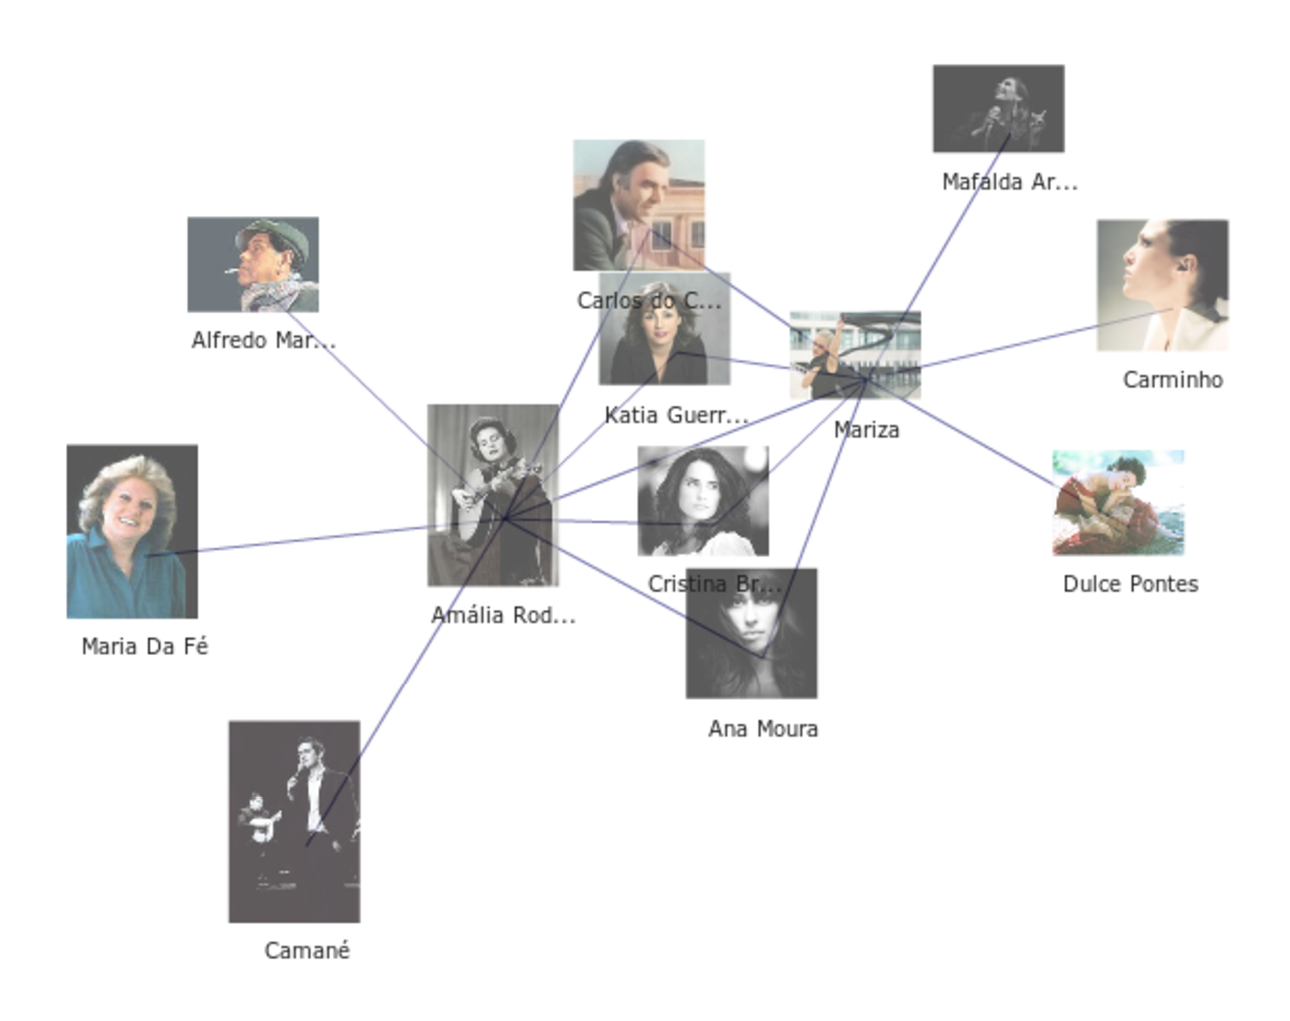
\includegraphics[width=\textwidth]{musicroamer4.pdf}
    \end{center}
    \caption{MusicRoamer: Grafo depois de expandir um nó}
    \label{fig:sota_musicroamer4}
  \end{figure}

  % subsubsection contras (end)

  \subsubsection{Resumo} % (fold)
  \label{ssub:resumo}

  Apesar de um utilizador do MusicRoamer ter muita liberdade na criação do grafo, a sua apresentação global é fraca e pouco trabalhada esteticamente.
  
  % subsubsection resumo (end)

% subsection musicroamer (end)


% section projetos_relacionados (end)


\section{Resumo e Conclusões}

Existem muitas outras ferramentas de descoberta de música. Apesar serem poucas as que usam esta representação visual em grafo, todas elas são importantes de se referir:

\begin{itemize}
  \item liveplasma.com
  \item audiomapa.tuneglue.net
  \item musicroamer.com
  \item discovr.info
  \item ifyoudig.net
  \item pitchfork.com
  \item hypem.com
  \item awdio.com
  \item 8tracks.com
  \item tastekid.com
  \item songza.com
  \item thesixtyone.com
  \item mog.com
  \item stereogum.com
  \item gigfi.com
  \item jango.com
  \item soundcloud.com
  \item grooveshark.com
\end{itemize}


Umas das primeiras lições que se tira dos exemplos dados é que quanto maior for o fator de ramificação de um grafo, mais confuso e saturado se torna.
Não é um exagero dizer que para além de confuso, o grafo perde o seu propósito inicial de ajudar o utilizador na sua descoberta de música nova.

Uma forma de evitar este problema, por exemplo, será limitar o fator de ramificação a um máximo que não cause este problema.
%!TEX root = ../report.tex

\chapter{Contextualization}
\label{chap:chap3}

\section*{}

The primal objective of this dissertation, as referred in chapter \ref{chap:intro}, is to develop one or more software modules that will improve Spotify users' music discovery and recommendation experience using visual tools to represent the music artists' relations and Spotify's streaming service to provide high quality music stream.

The initial proposal was to develop a module that implements, at least, one of the following features:

\begin{enumerate}
  \label{chap3:modules}
  \item \label{item:obj1} Integrate Spotify's music stream into RAMA's website
  \item \label{item:obj2} Integrate information from the Spotify user into RAMA
  \item \label{item:obj3} Improve RAMA's features and design
  \item \label{item:obj4} Integrate the RAMA concept into a Spotify Application
  \item \label{item:obj5} Integrate RAMA's playlist generation into a Spotify Application
  \item \label{item:obj6} Integrate some of the above mentioned modules into a Mobile Application
\end{enumerate}

The first three functionalities (\ref{item:obj1}, \ref{item:obj2} and \ref{item:obj3}) focus on improving RAMA using Spotify's API, i.e. to integrate Spotify into RAMA.
Whereas \ref{item:obj4} and \ref{item:obj5} aim to integrate RAMA's concept into Spotify, through a Spotify Application (it would work as a plugin to Spotify's Desktop Client).
The last one (\ref{item:obj6}) would focus on implementing the previous functionalities into an Android, iOS or Windows Phone Application.
The aim of this chapter is to compare and contrast these proposed features, towards determining which among them will be pursued in this thesis, either: Spotify Application, Mobile Application, or RAMA improvements.

At first, Spotify's user environment will be introduced (\ref{sec:spotify}), followed by Spotify's Development Tools (\ref{sec:devtools}) in order to assess which tools are available for developers.
Next, the available tools will be evaluated, through experiments (\ref{sec:experiments}), in order to determine which ones fit the proposed modules better.

By the end of this chapter the modules developed should be clearly stated, as well as which development tools will be used in the prototype.
The prototype should pursue the objective of contributing to an improved user experience of discovering new music by taking advantage of visual tools that implement RAMA's concept.

\section{Introducing Spotify} % (fold)
\label{sec:spotify}

  % 

  Spotify is a Music Streaming Service that allows the user, through an Internet connection, to listen to any track (if available in the user's country) in Spotify's catalogue.
  The service was launched in 2008 with a native desktop client application.
  Now, the service has several types of clients available to the users: desktop client, webplayer and mobile applications.

  \begin{description}
    \item[\textbf{Desktop Client}] Desktop version of Spotify, with Windows and Mac versions (and also a Linux preview version).
    \item[\textbf{Webplayer}] Web version of Spotify. This was released in 2013, although Spotify still advises the use of the native application for a better user experience.
    \item[\textbf{Mobile Applications}] The mobile applications are available for Android and iOS devices.
  \end{description}

  % \subsection{Music Discovery Tools} % (fold)
  % \label{sub:discovery_tools}
  
  % browse: groups of playlists
  % activity: social side that shows the user's friends' activity on spotify (what they listen to)
  % discover: artists/albums/tracks suggestions based on the user's listening history.
  % top lists: 2


  % subsection discovery_tools (end)


  \section{Development Tools} % (fold)
  \label{sec:devtools}
  
    Spotify provides a set of tools\footnote{\url{http://developer.spotify.com/technologies}} to develop Third-party Applications (websites, native applications and mobile applications) and Spotify Applications (that run inside Spotify's Desktop Client).
    There are five tools, each with different purposes.

    \subsection{Spotify Applications} % (fold)
    \label{sub:spotify_apps}
      Spotify Applications~\cite{spotifyapps} are a special case in the whole set of tools provided by Spotify.
      These applications are designed to run \emph{inside} the Desktop Client.
      Spotify users can run and install applications from the store called ``App Finder''.
      All the applications are free.
      In Figure~\ref{fig:spotify_apps} one can see the interface of the desktop client.
      In this case, the discovery mode's interface.
      \begin{figure}
        \begin{center}
          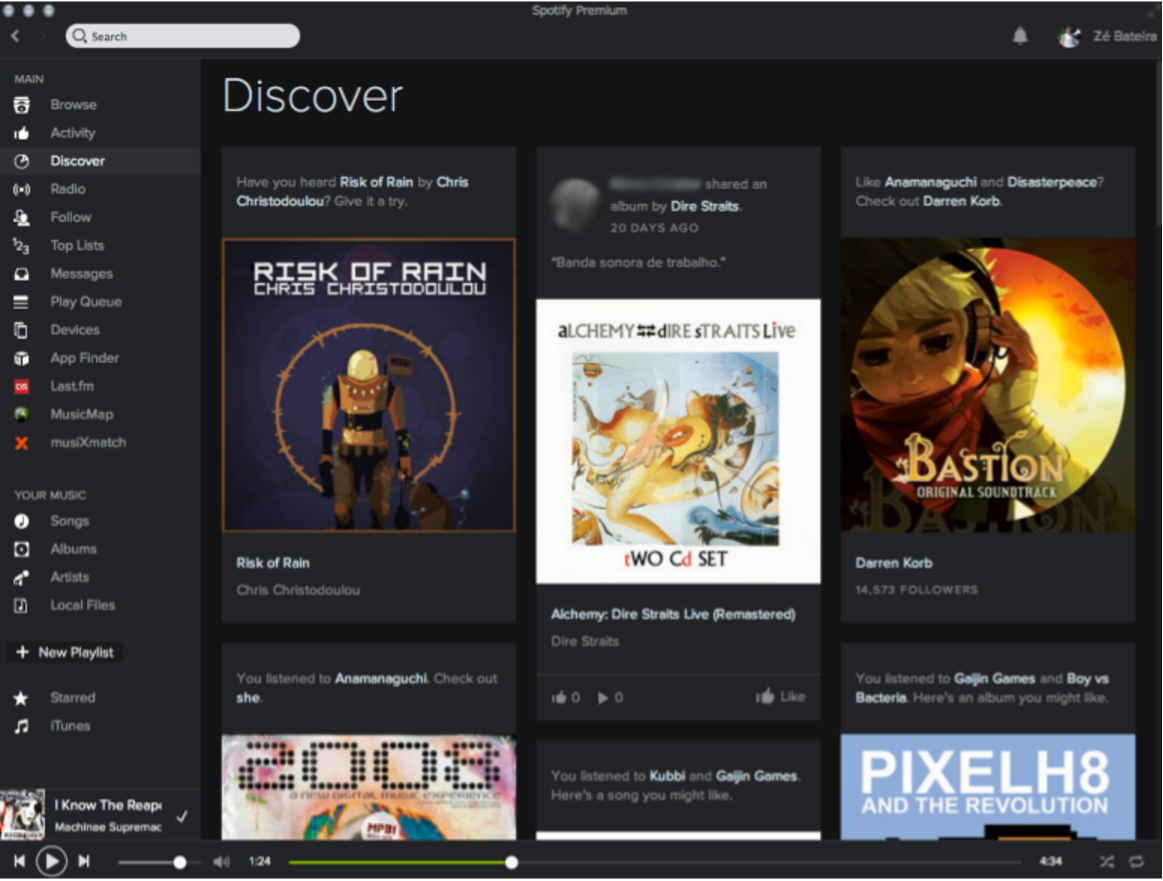
\includegraphics[width=\textwidth]{spotify_discovery.mode.pdf}
        \end{center}
        \caption{Spotify: desktop client's discovery mode interface.}
        \label{fig:spotify_apps}
      \end{figure}
      On the left side, in the menu, bellow the ``App Finder'' item, appears all the applications the user as installed from the store.
      In Figure~\ref{fig:spotify_apps2} the official Last.fm application is opened.
      Note how the space filled by the applications is always the same.

      \begin{figure}
        \begin{center}
          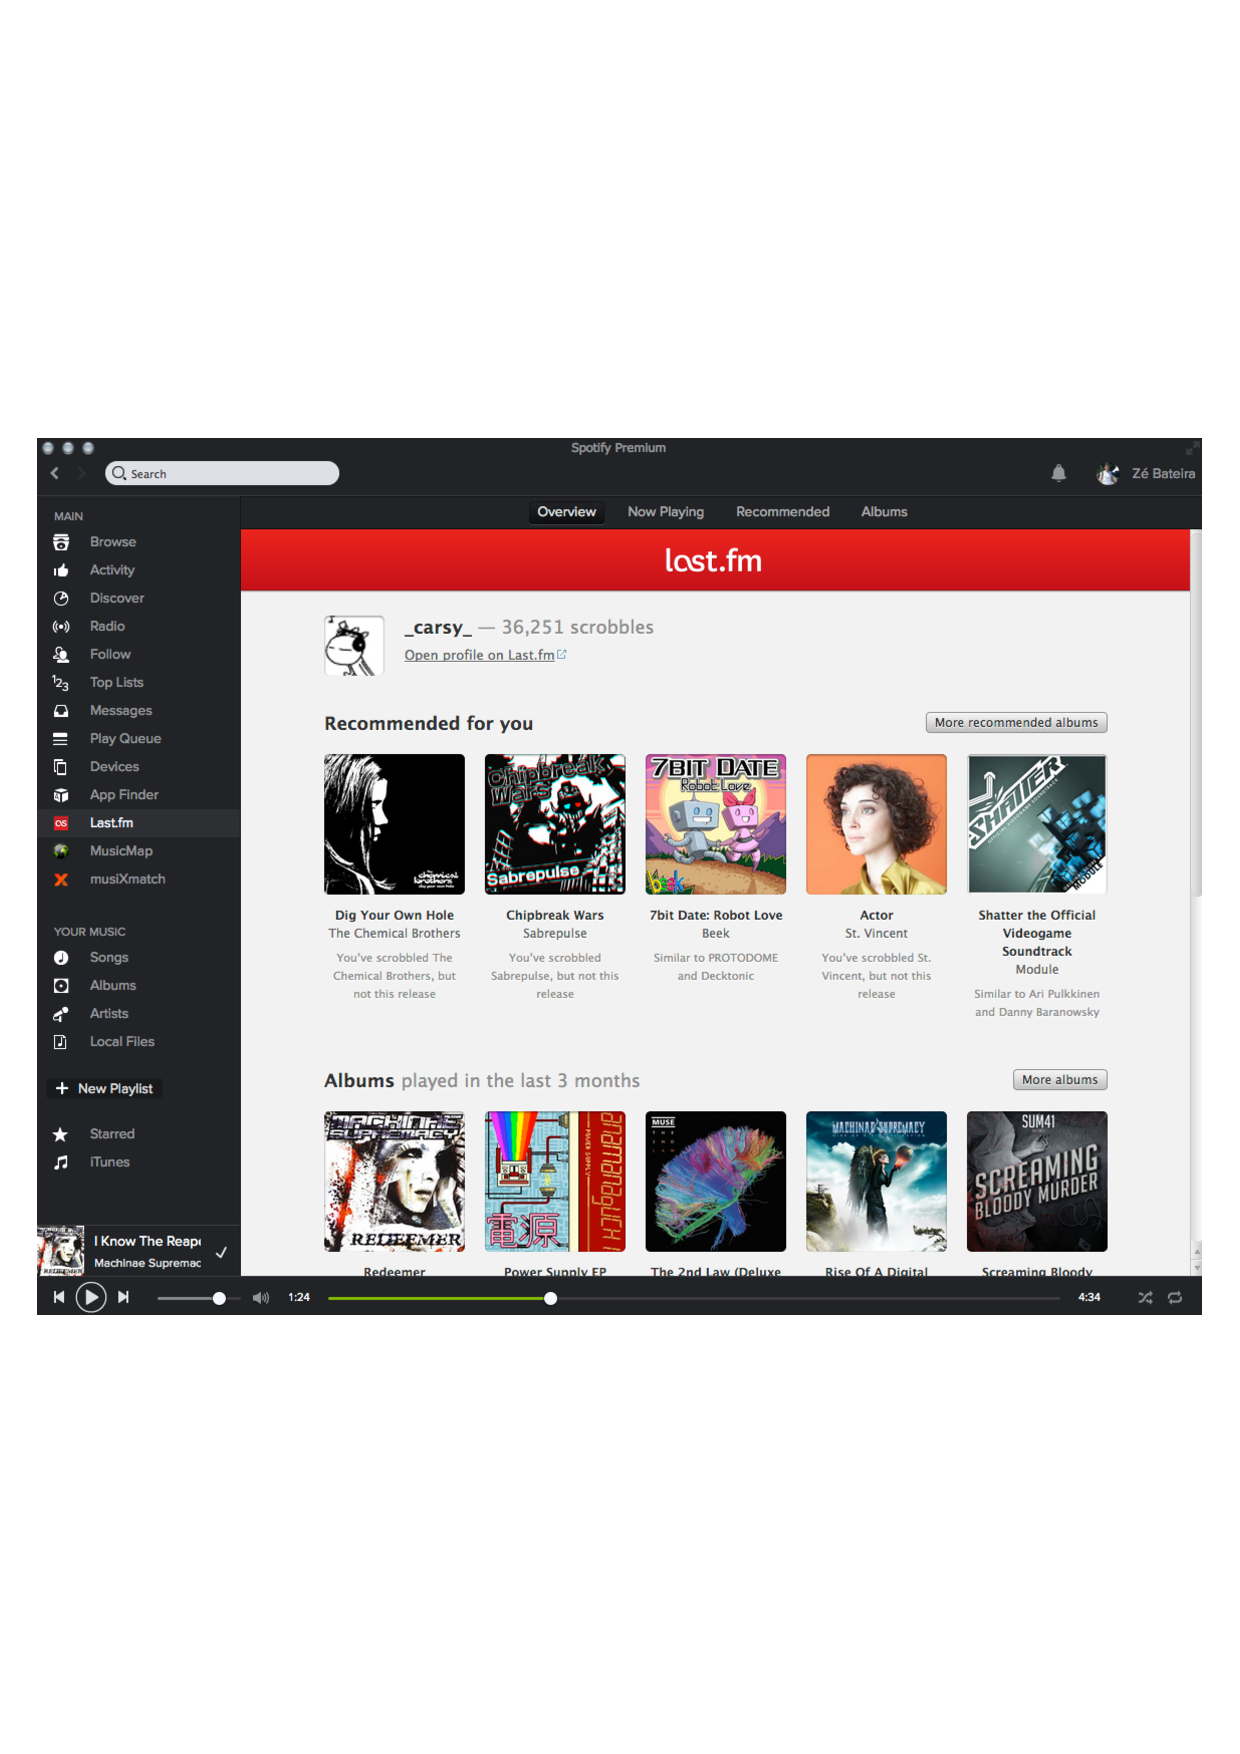
\includegraphics[width=\textwidth]{spotify_apps.pdf}
        \end{center}
        \caption{Spotify: Last.fm's Spotify Application opened.}
        \label{fig:spotify_apps2}
      \end{figure}

      The Applications' runtime environment is one of a browser-based.
      More specifically, powered by the Chromium Embedded Framework~\cite{chromiumembedded}.
      This means that the code to develop a Spotify Application follows the same principles as a web application: HTML, CSS and Javascript.

      Spotify developed two Frameworks\footnote{\url{https://developer.spotify.com/technologies/apps/reference}} to help developers create these applications: the API 1.x Framework\footnote{\url{https://developer.spotify.com/docs/apps/api/1.0/}} and the Views Framework\footnote{\url{https://developer.spotify.com/docs/apps/views/1.0/}}.
      The first one provides an interface to use object models, access metadata, control the player, among others.
      The second offers support for web components like buttons, lists, tabs, among others.

    % subsubsection spotify_apps (end)


    \subsection{Spotify Widgets} % (fold)
    \label{sub:spotify_widgets}

      Spotify Widgets~\cite{spwidgets} are small web components that can be embedded in external websites.
      Spotify provides two components: \emph{Play Button} (Figure~\ref{fig:spotify_play_button}) and a \emph{Follow Button} (Figure~\ref{fig:spotify_follow_button})

      \begin{figure}[H]
        \begin{center}
          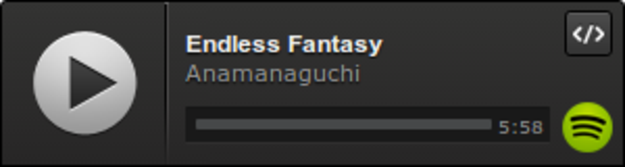
\includegraphics[width=0.5\textwidth]{spotify_play_button.pdf}
        \end{center}
        \caption{Spotify: \emph{Play Button}.}
        \label{fig:spotify_play_button}
      \end{figure}

      \begin{figure}[H]
        \begin{center}
          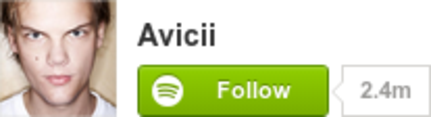
\includegraphics[width=0.5\textwidth]{spotify_follow_button.pdf}
        \end{center}
        \caption{Spotify: \emph{Follow Button} Allows the user to follow the music artist.}
        \label{fig:spotify_follow_button}
      \end{figure}

      However, there are some limitations.
      In Spotify, only logged in users can use the service (listen to tracks, etc).
      This also applies to these widgets - even if they are in an external application, only Spotify users can interact with them.
      This limitation does make sense in the case of the \emph{Follow Button}, but the \emph{Play Button} becomes useless to non-Spotify users.
      In truth, these widgets are nothing but a hyperlink to a Spotify Client (Web Player or Desktop).
      With the Play Button, the stream of tracks always plays inside Spotify's environment, and not on external applications.

      To embed a widget, it is only required to copy-paste Html code into the website, where appropriate:

      \lstinputlisting[language=HTML,caption={Html code to embed the \emph{Play Button}}, style=htmlcssjs, captionpos=b]{snippets/play_button.html}

      These widgets are useful to develop the proposed modules \ref{item:obj1} and \ref{item:obj3}.

    % subsubsection spotify_widgets (end)

    \subsection{Libspotify SDK} % (fold)
    \label{sub:libspotify_sdk}

      Libspotify SDK~\cite{libspotifysdk} is an API that allows for third-party applications to include Spotify's services into them.
      However, not without some limitations to the users of these applications.
      The users are limited depending on the type of Spotify Subscription that they have signed up to.

      There are three different types of subscriptions~\cite{spsubscription}, but the important part to retain, is the difference between being a Free Subscription Spotify User, and a Paid Subscription Spotify User (premium and unlimited subscriptions).
      As mentioned before, only Spotify users can interact with Spotify Widgets (Figure~\ref{sub:spotify_widgets}).
      That also applies to third-party applications that are using Libspotify SDK, which allow, for example, the user to login with their Spotify account.
      But in this case, not only do they need to be Spotify users, they also need to have signed up to a paid Spotify subscription.
      And not only do the users need to pay to use the Spotify-powered application, but the developers as well.
      This is a very restrictive environment, although Libspotify SDK comes in many different flavours~\cite{libspotifysdkdown}.

      This tool would be used to develop modules \ref{item:obj1}, \ref{item:obj2} and \ref{item:obj6}.
      

    % subsubsection libspotify_sdk (end)


    \subsection{Metadata API} % (fold)
    \label{sub:metadata_api}

      The \emph{Metadata API}\footnote{This API was very recently deprecated (June, 2014) and was replaced by the \emph{Web API}. It follows the same principles of the previous one, and so, for the purposes of this report, the differences are not relevant.}~\cite{spmetadata} allows for applications to retrieve information from Spotify's music catalogue: tracks, albums, artists, playlists, and so on.

      Requests to the database are done through HTTP and are of two types: \emph{search}\footnote{\url{https://developer.spotify.com/technologies/web-api/search}} e \emph{lookup}\footnote{\url{https://developer.spotify.com/technologies/web-api/lookup}}.
      To request detailed information of, e.g., an artist, the URI (used as the unique identifier) of that artist is required. Such ID is of the form:

      \url{spotify:artist:<artist_id>}, where \emph{artist\_id} is the unique identifier of the artist.

      Example:

      \url{spotify:artist:65nZq8l5VZRG4X445F5kmN}, is the ID for the artist ``Mariza''. \\

      There are also ID's for albums:

      \url{spotify:album:5d1LpIPmTTrvPltx26TlEU} (album ``Fado Tradicional'' from ``Mariza'') \\

       and for tracks:

       \url{spotify:track:2vqYasauhDLVjTt7CGWK6y} (track ``Fado Vianinha'' of the previous album) \\

      These URI schemes are compliant with Rosetta Stone's ID spaces~\cite{rosettastone}.

      First, to get this URI, one needs to search the database.

      \begin{description}
        \item[\emph{Search}] \hfill

          The base \emph{URL}:

          \url{http://ws.spotify.com/search/1/album}, to search for albums.

          For artists, \emph{artist}, for tracks, \emph{track}. \\

          Examples:

          \url{http://ws.spotify.com/search/1/album?q=foo} \\
          \url{http://ws.spotify.com/search/1/artist.json?q=red+hot} \\

          The request response, by default, is formatted in \emph{XML}, although, as the second example demonstrates, \emph{JSON} is also supported.

          Given the following query: \\
          \url{http://ws.spotify.com/search/1/artist.json?q=camane}

          The server responds with:

          \lstinputlisting[caption={Results ordered by ``popularity''}, style=htmlcssjs, captionpos=b]{snippets/search_camane.json}

        \item[\emph{Lookup}] \hfill \\

          When the URI is known, one can finally lookup detailed information about a database item. With the following query:

          \sloppy
          \url{http://ws.spotify.com/lookup/1/.json?uri=spotify:artist:3MLPFTe4BrpEV2eOVG0gLK&extras=album}

          The server responds with:

          \lstinputlisting[caption={\emph{lookup} of the artist ``Camané''}, style=htmlcssjs, captionpos=b]{snippets/lookup_camane.json}

      \end{description}

      This API is very useful for all the six proposed modules.

    % subsubsection metadata_api (end)

    \subsection{iOS SDK (beta)} % (fold)
    \label{sub:ios_sdk}
    
    The iOS SDK supports iOS Application developers. Although still in beta~\cite{iossdk}, this tool would be used to develop the proposed module \ref{item:obj6}.
    Much like the Libspotify SDK, this SDK provides the following APIs:

    \begin{itemize}
      \item User authentication
      \item Audio playback and stream management
      \item Metadata (artist, album, track) lookup including artwork
      \item Playlist management
    \end{itemize}

    % subsubsection ios_sdk (end)

  % subsection devtools (end)

  \section{Experiments} % (fold)
  \label{sec:experiments}

    As a first hands-on experience with these tools, a single-page website was developed which allows the users to search and listen to music using Spotify's \emph{Metadata API} and \emph{Widgets}: \\

    \url{http://carsy.github.io/spotify-playground} \\

    In Figure~\ref{fig:playground} one can see a search result and the \emph{Widget Play Button} with the selected item.

    \begin{figure}
      \centering

      \begin{subfigure}{0.38\textwidth}
        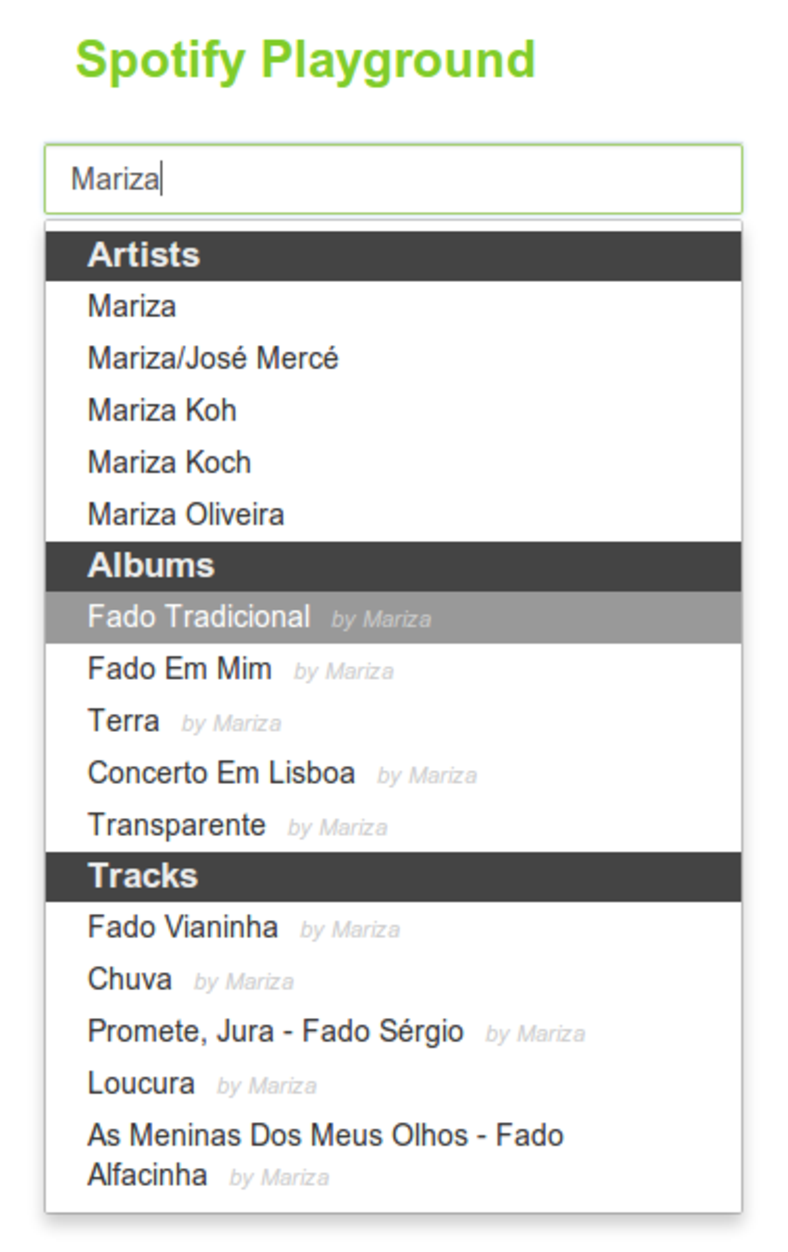
\includegraphics[width=\textwidth]{playground.pdf}
        \caption{Search result for ``Mariza''}
        \label{fig:playgroun_a}
      \end{subfigure}

      \begin{subfigure}{0.38\textwidth}
        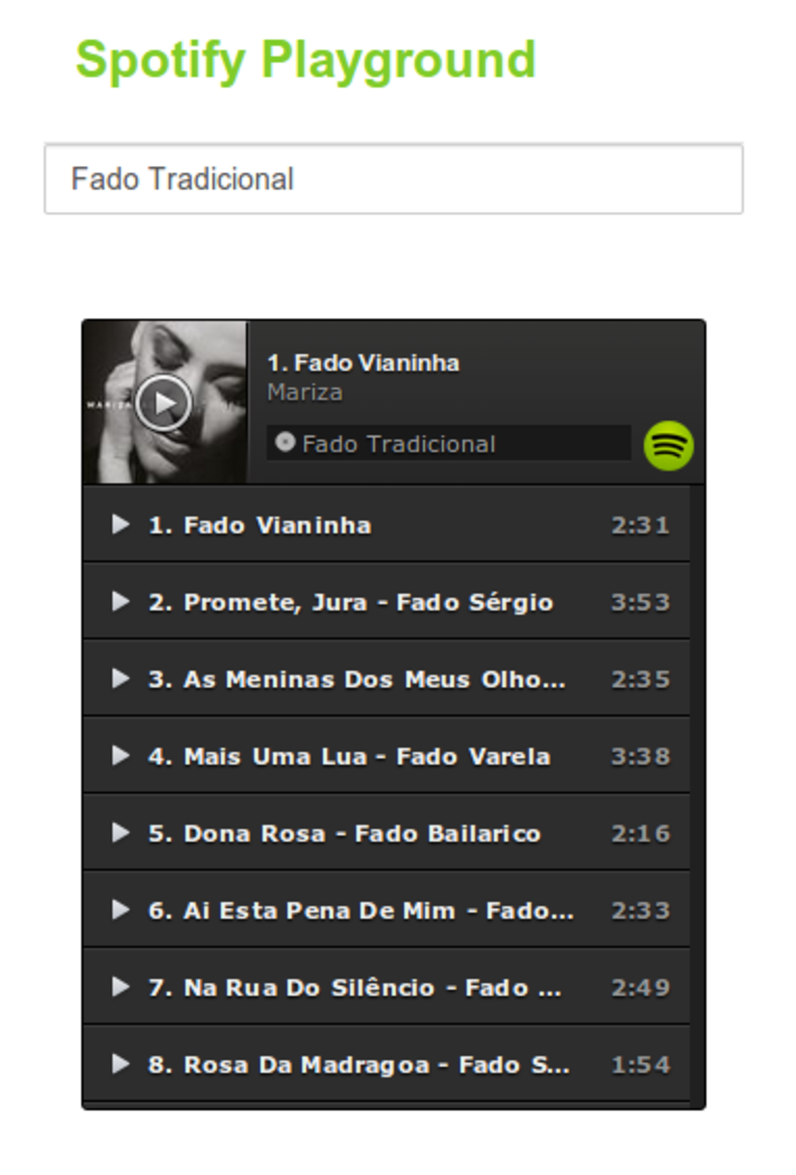
\includegraphics[width=\textwidth]{playground2.pdf}
        \caption{After selecting the album ``Fado Tradicional'' the \emph{Play button} displays all of the album's tracks to be played in sequence.}
        \label{fig:playground_b}
      \end{subfigure}

      \caption{Experiment with the \emph{Metadata API} and the \emph{Play Button Widget} (source code: \url{github.com/carsy/spotify-playground})}
      \label{fig:playground}

    \end{figure}

    Both tools turned out to be well documented and easy to use.

    \clearpage

    Another experiment was made in order to assert the potential of Spotify Applications.
    There was a need to know if the canvas element was well supported by Spotify's environment, because that is the preferred way to graphically draw a graph.
    To test that, a simple application was created with the following code:

    \begin{lstlisting}[caption={\emph{iframe} element that allows to embed RAMA's website into the application.}, style=htmlcssjs, captionpos=b]
      <iframe src="http://rama.inescporto.pt/app" frameborder="0">
      </iframe>\end{lstlisting}

    The final result can be seen in Figure~\ref{fig:rama_spotifyed}.
    \begin{figure}[H]
      \begin{center}
        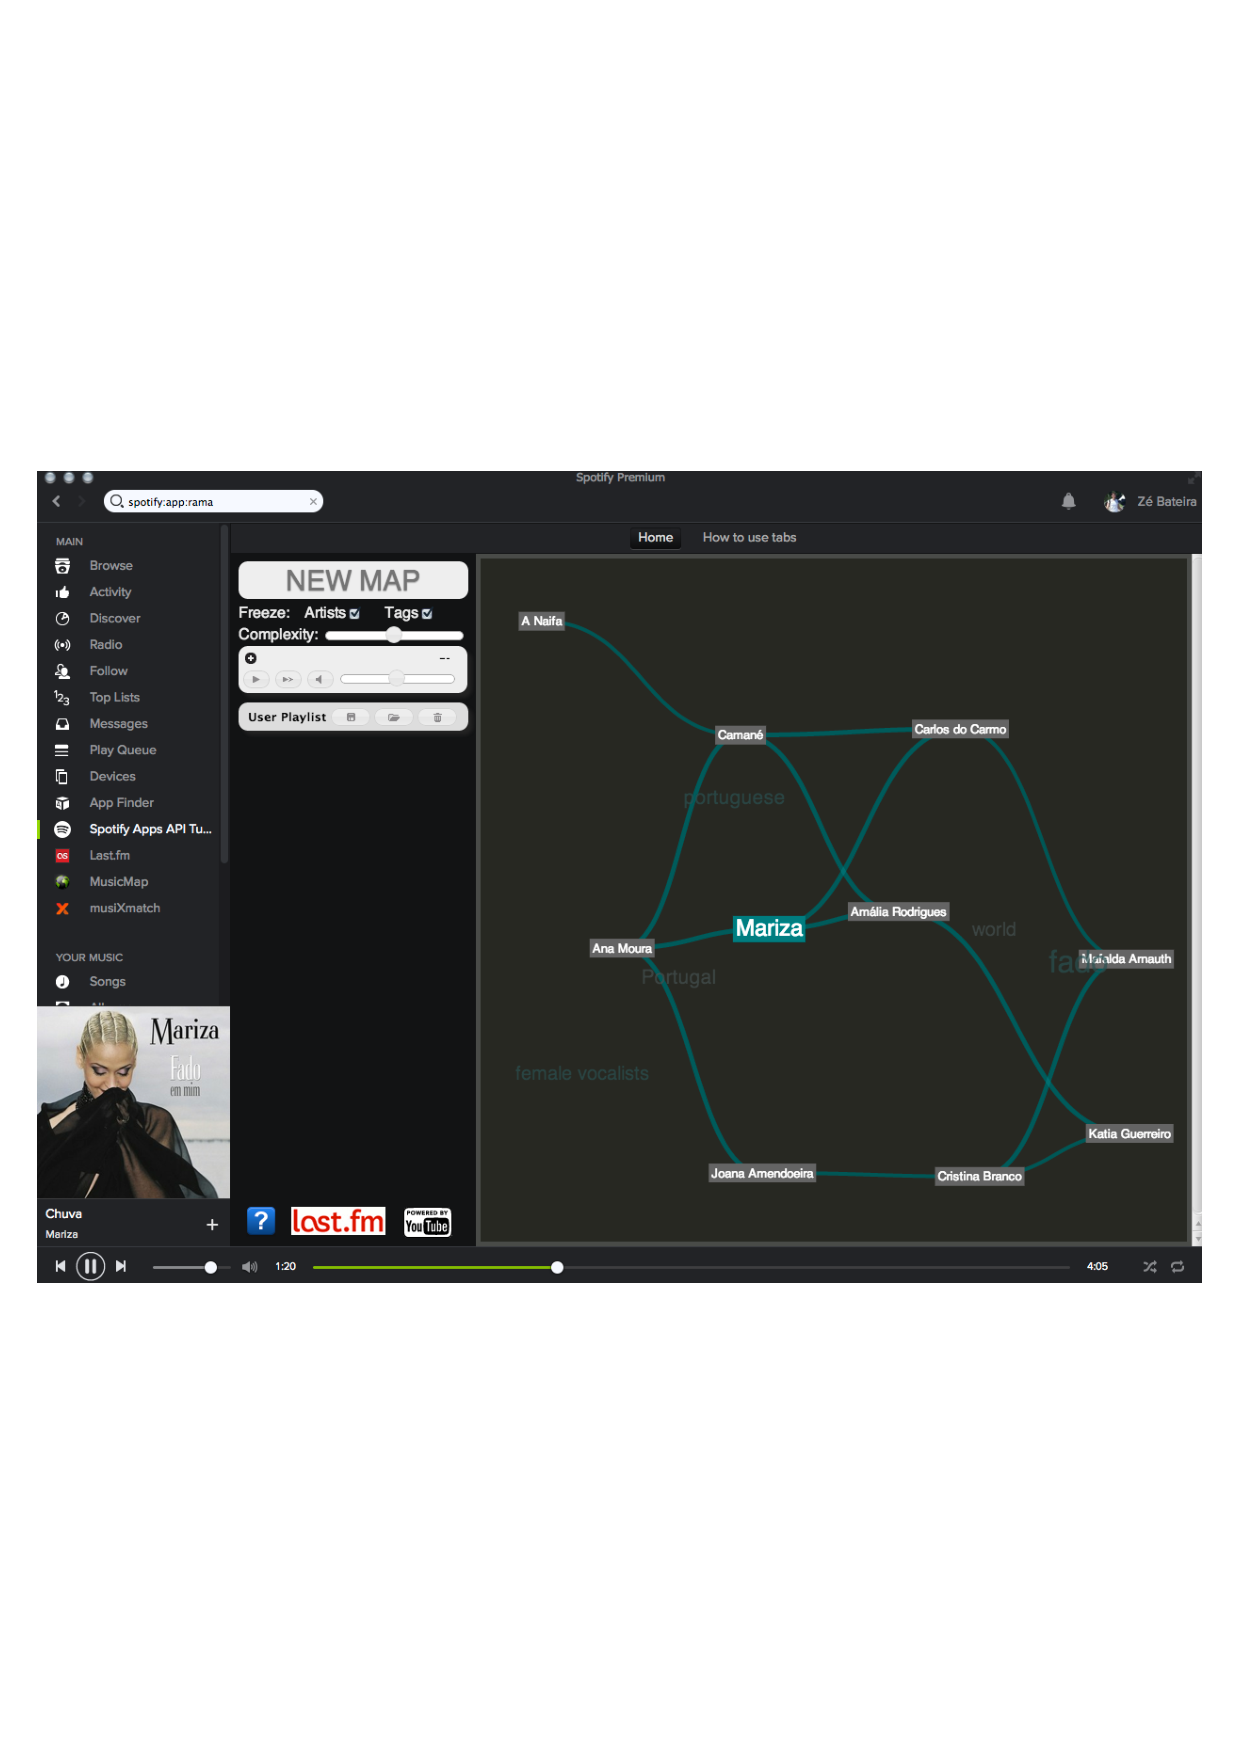
\includegraphics[width=\textwidth]{spotify_rama.embedded.pdf}
      \end{center}
      \caption{RAMA's website embedded into a Spotify Application.}
      \label{fig:rama_spotifyed}
    \end{figure}
    Although the \emph{iframe} and \emph{canvas} elements are supported, there are some that are not.
    This specific application is not usable since, for example, playing tracks from external sources is not allowed.
    Nonetheless, there is a way to test which HTML elements are supported, using an internal Spotify application.
    In Figure~\ref{fig:canvas_support} one can see the 100\% supported canvas element.

    \begin{figure}[H]
       \begin{center}
         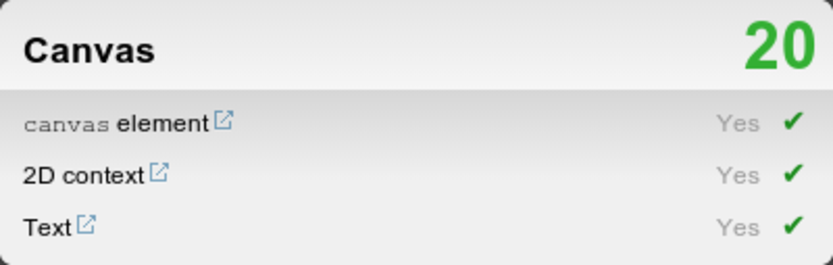
\includegraphics[width=0.5\textwidth]{canvas_support.pdf}
       \end{center}
       \caption{Test result for the canvas element.}
       \label{fig:canvas_support}
     \end{figure}

  % subsection experiments (end)

% section spotify (end)

\section{Summary}

  Based on the analysis conducted, the most appropriate solution was to develop a Spotify Application.
  Although the other proposals were also feasible, the possibility to integrate a RAMA-like interface into Spotify's Desktop Client leaves a Spotify user more at ease with the environment.
  The prototype should then implement the proposed modules \ref{item:obj4} and \ref{item:obj5}:

  \begin{itemize}
    \item[4.] Integrate the RAMA concept into a Spotify Application
    \item[5.] Integrate RAMA's playlist generation into a Spotify Application
  \end{itemize}

%!TEX root = ../report.tex


\chapter{Implementation and Validation}
\label{chap:chap4}

\section*{}

In this chapter, further details about the methodologies used in the developed prototype, as well as in the the validation process, will be explored.

The Development Processes section will go into details about the processes used to maintain a sane development environment by taking advantage of several tools that automated most of the common tasks.

By this point, the validation of the prototype will be analysed, by explaining the performed user tests, as well the analysis of the results.


\section{Prototype} % (fold)
\label{sec:prototype}

  \subsection{Main Features} % (fold)
    \label{sub:main_features}
    
    The main features of RAMA's Spotify Application are: visualization of a map of a network of connected artists; edition of the visualization parameters; edition of the graph (expand and new map functions); Tags overlay and music artist info.

    \subsubsection{Visulization of the Artists Map} % (fold)
      \label{ssub:visualization}
    
      The application automatically draws the map with the current playing artist as the main node, as seen in Figure~\ref{fig:graph_rootnode}.

      \begin{figure}[tb]
        \begin{center}
          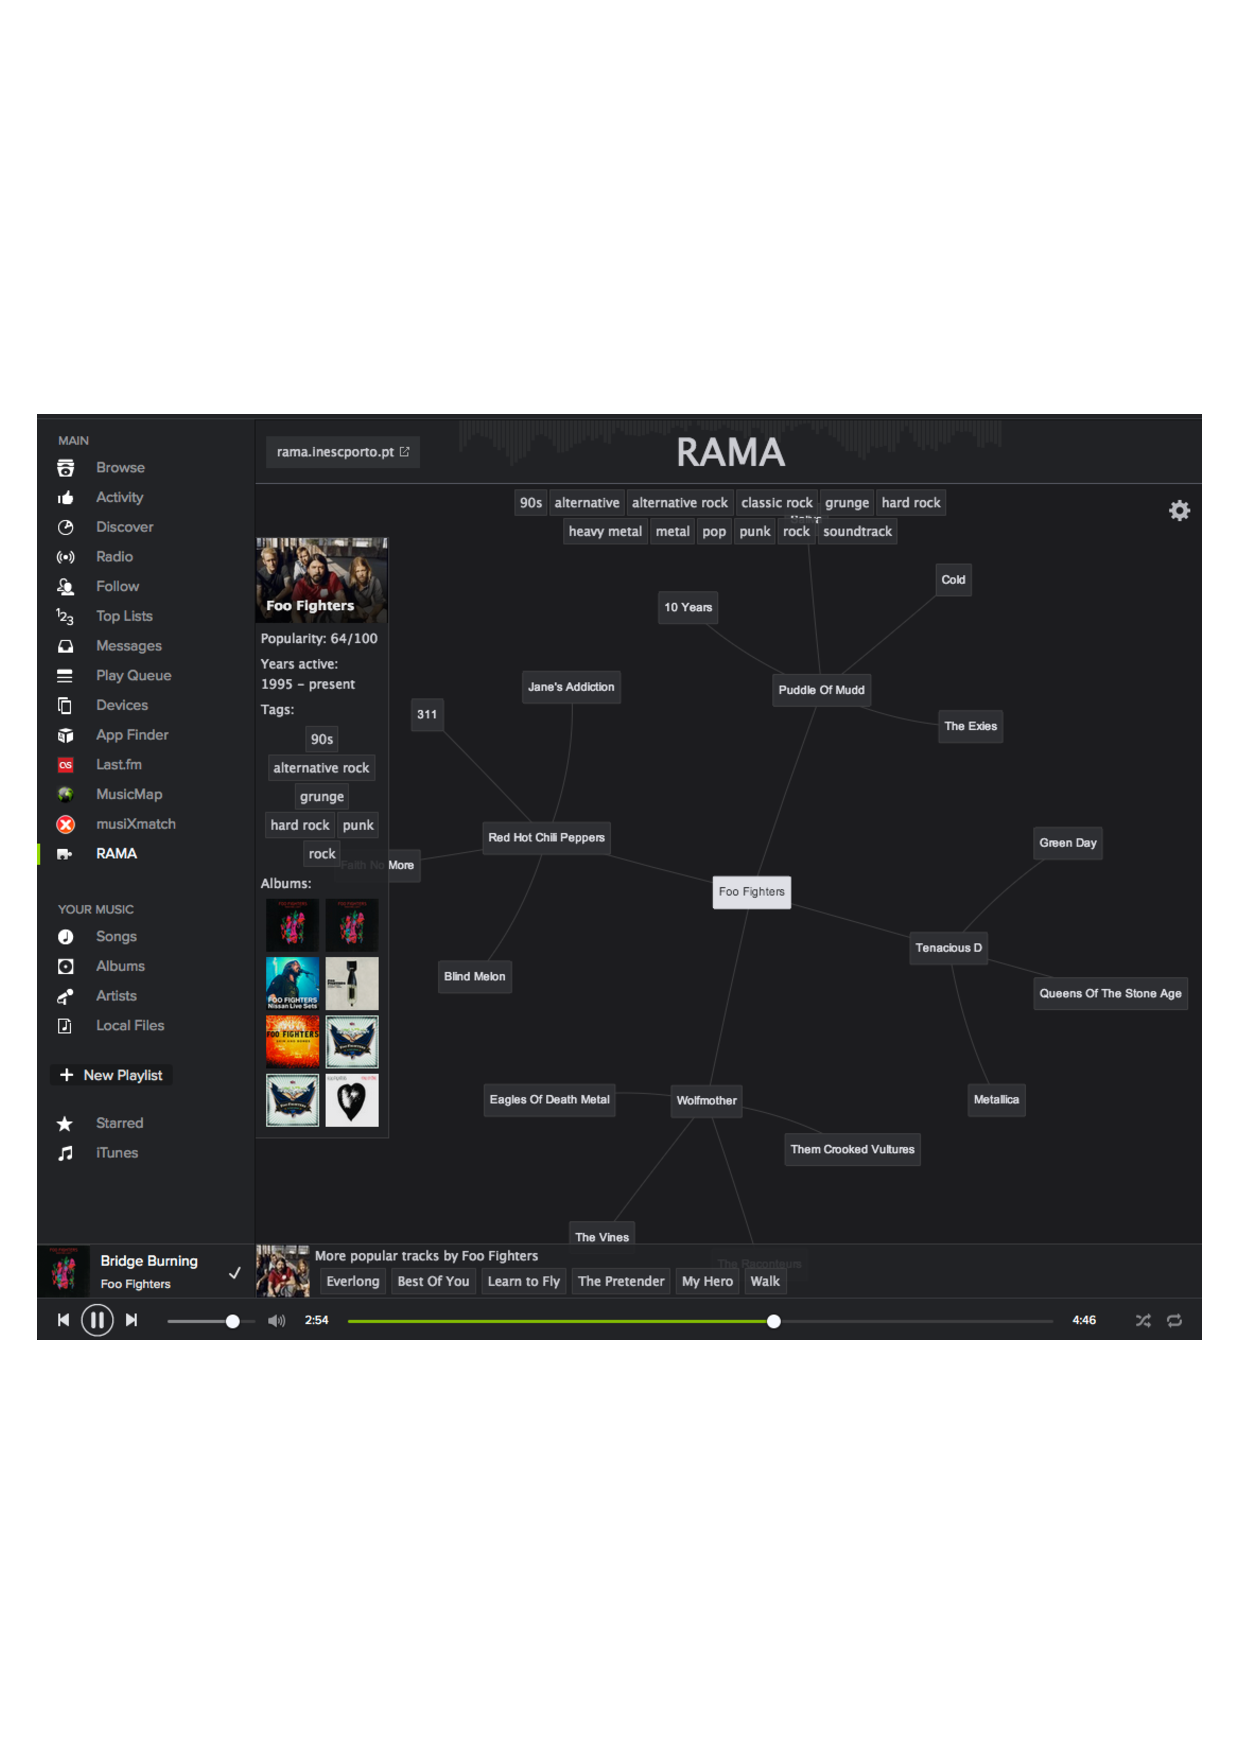
\includegraphics[width=\textwidth]{graph_rootnode.pdf}
        \end{center}
        \caption{The first drawn graph uses the current playing artist (lower left corner) as the root node.}
        \label{fig:graph_rootnode}
      \end{figure}

      The graph-like structure is created by recursively fetching a list of related artists from each artist. Once a certain pre-established limit of recursive levels is reached\footnote{depth value of a graph}, the algorithm stops.

      The graph creation algorithm is as follows:

      % change the code the attachments
      \lstinputlisting[
        caption={Simplified graph creation algorithm in Javascript (duplicate nodes checking is encapsulated in the insertNode function)}, style=htmlcssjs
      ]
      {snippets/map_creation_alg.js}

      This algorithm, albeit simplified, represents the basic flow when constructing a graph, or more specifically, a tree.
      Since that, in this case of study, the direction of the edges of the graph is not relevant in any way to the artists' map, all of the edges are considered to be undirected.

      Assuming that the insertNode() function checks for duplicate nodes, i.e., it only inserts unique nodes into the graph, then the resulting graph is one of a tree, since there are no simple cycles in the graph.
      An example of this behaviour can be seen in Figure~\ref{fig:graph_treemode}.

      \begin{figure}[tb]
        \begin{center}
          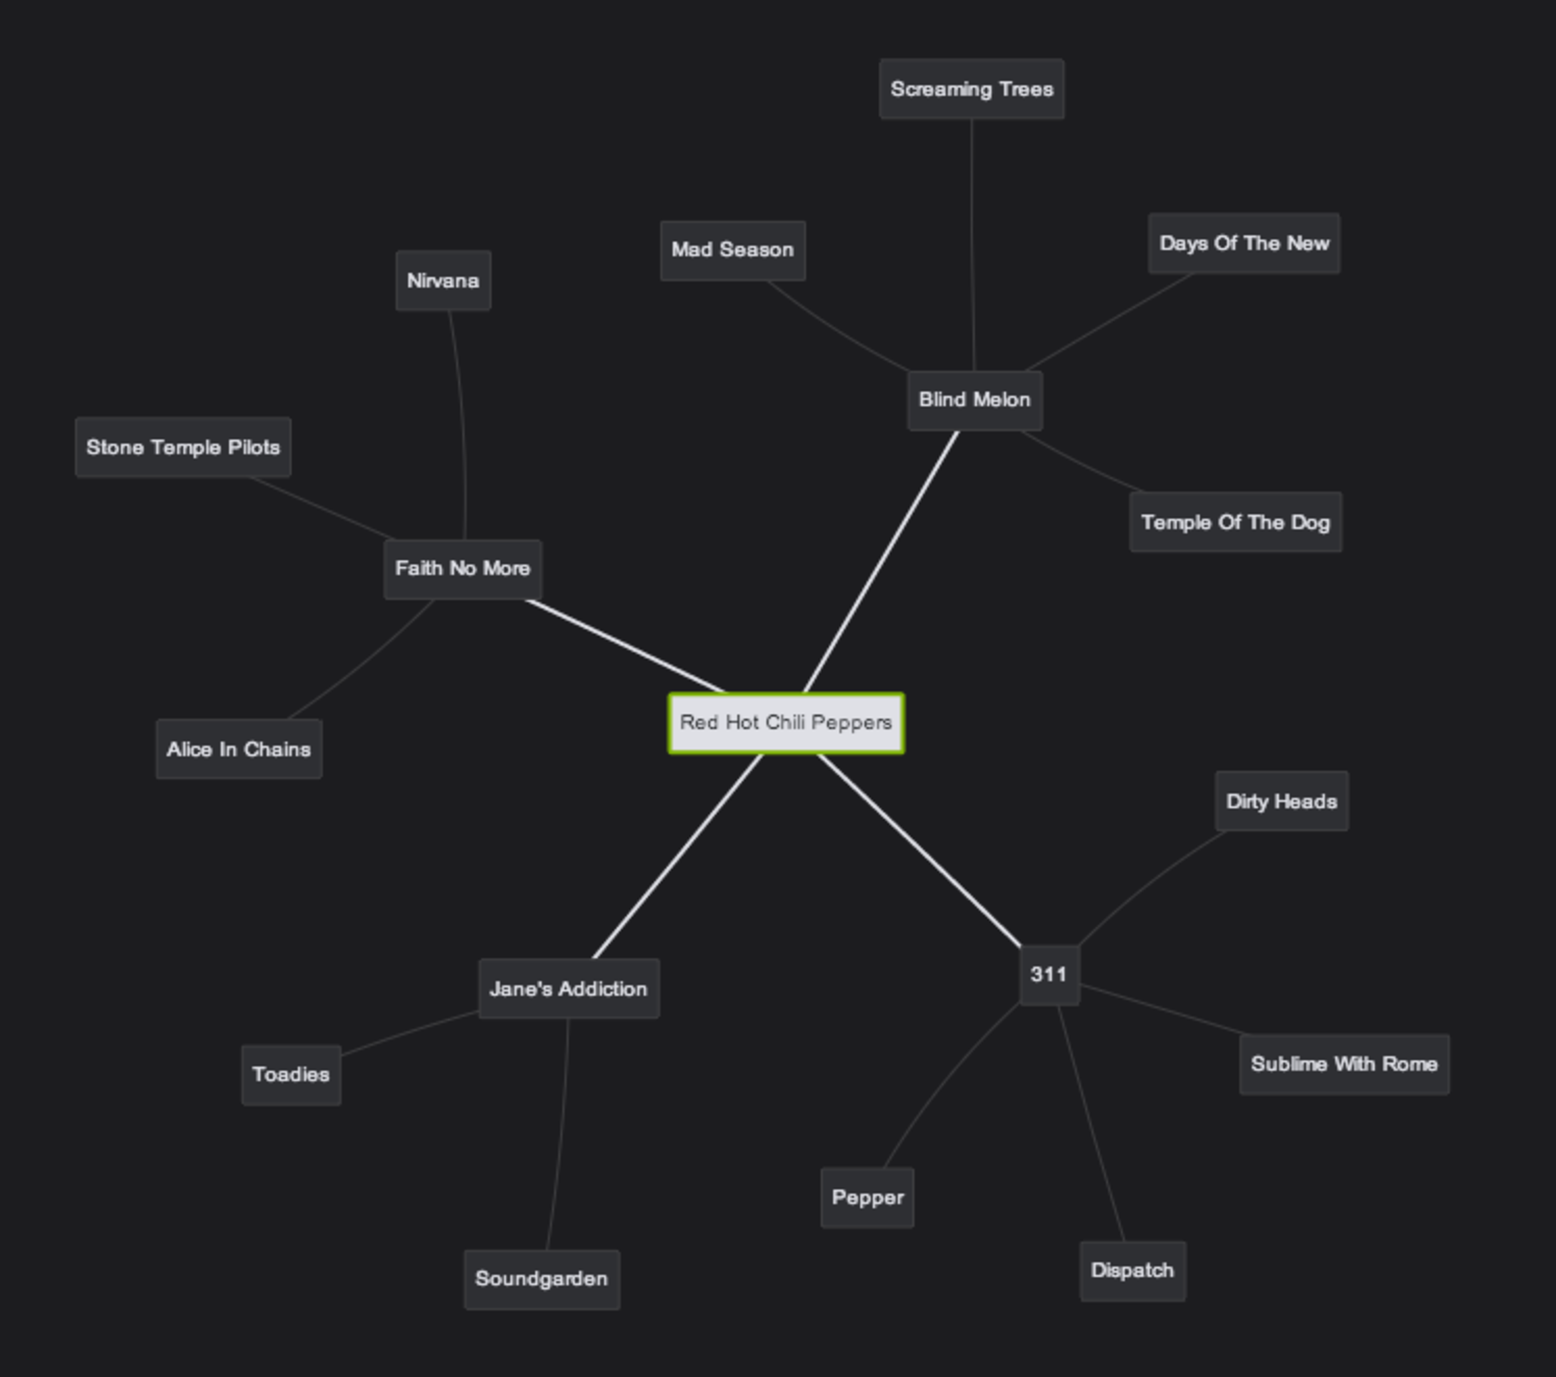
\includegraphics[width=\textwidth]{map_creation_treemode.pdf}
        \end{center}
        \caption{Graph created like a tree with "Red Hot Chilli Peppers" as the root node.}
        \label{fig:graph_treemode}
      \end{figure}

      This approach, however, is not showing all of the available information.
      Given this same example (Figure~\ref{fig:graph_treemode}), the artist node "Stone Temple Pilots" is a child of the node artist "Faith No More".
      The algorithm inserted the latter first into the graph.
      After that, when retrieving the childs of "Jane's Addiction", "Stone Templo Pilots" is contained in that list, and so the insertNode() function discards the node since it is a duplicate.
      But that means that there is a connection between the both of them that is being discarded.

      \paragraph{Graph's Tree Mode} \hfill \\
      To build a graph with all the connections that exist between all of the artists in the graph, the insertNode() function would need to insert the missing edge into the graph by analysing the current graph state.
      This method creates a graph by definition, while the previous one created a tree graph.
      An example of this behaviour can be seen in Figure~\ref{fig:graph_notreemode}.
      \begin{figure}[tb]
        \begin{center}
          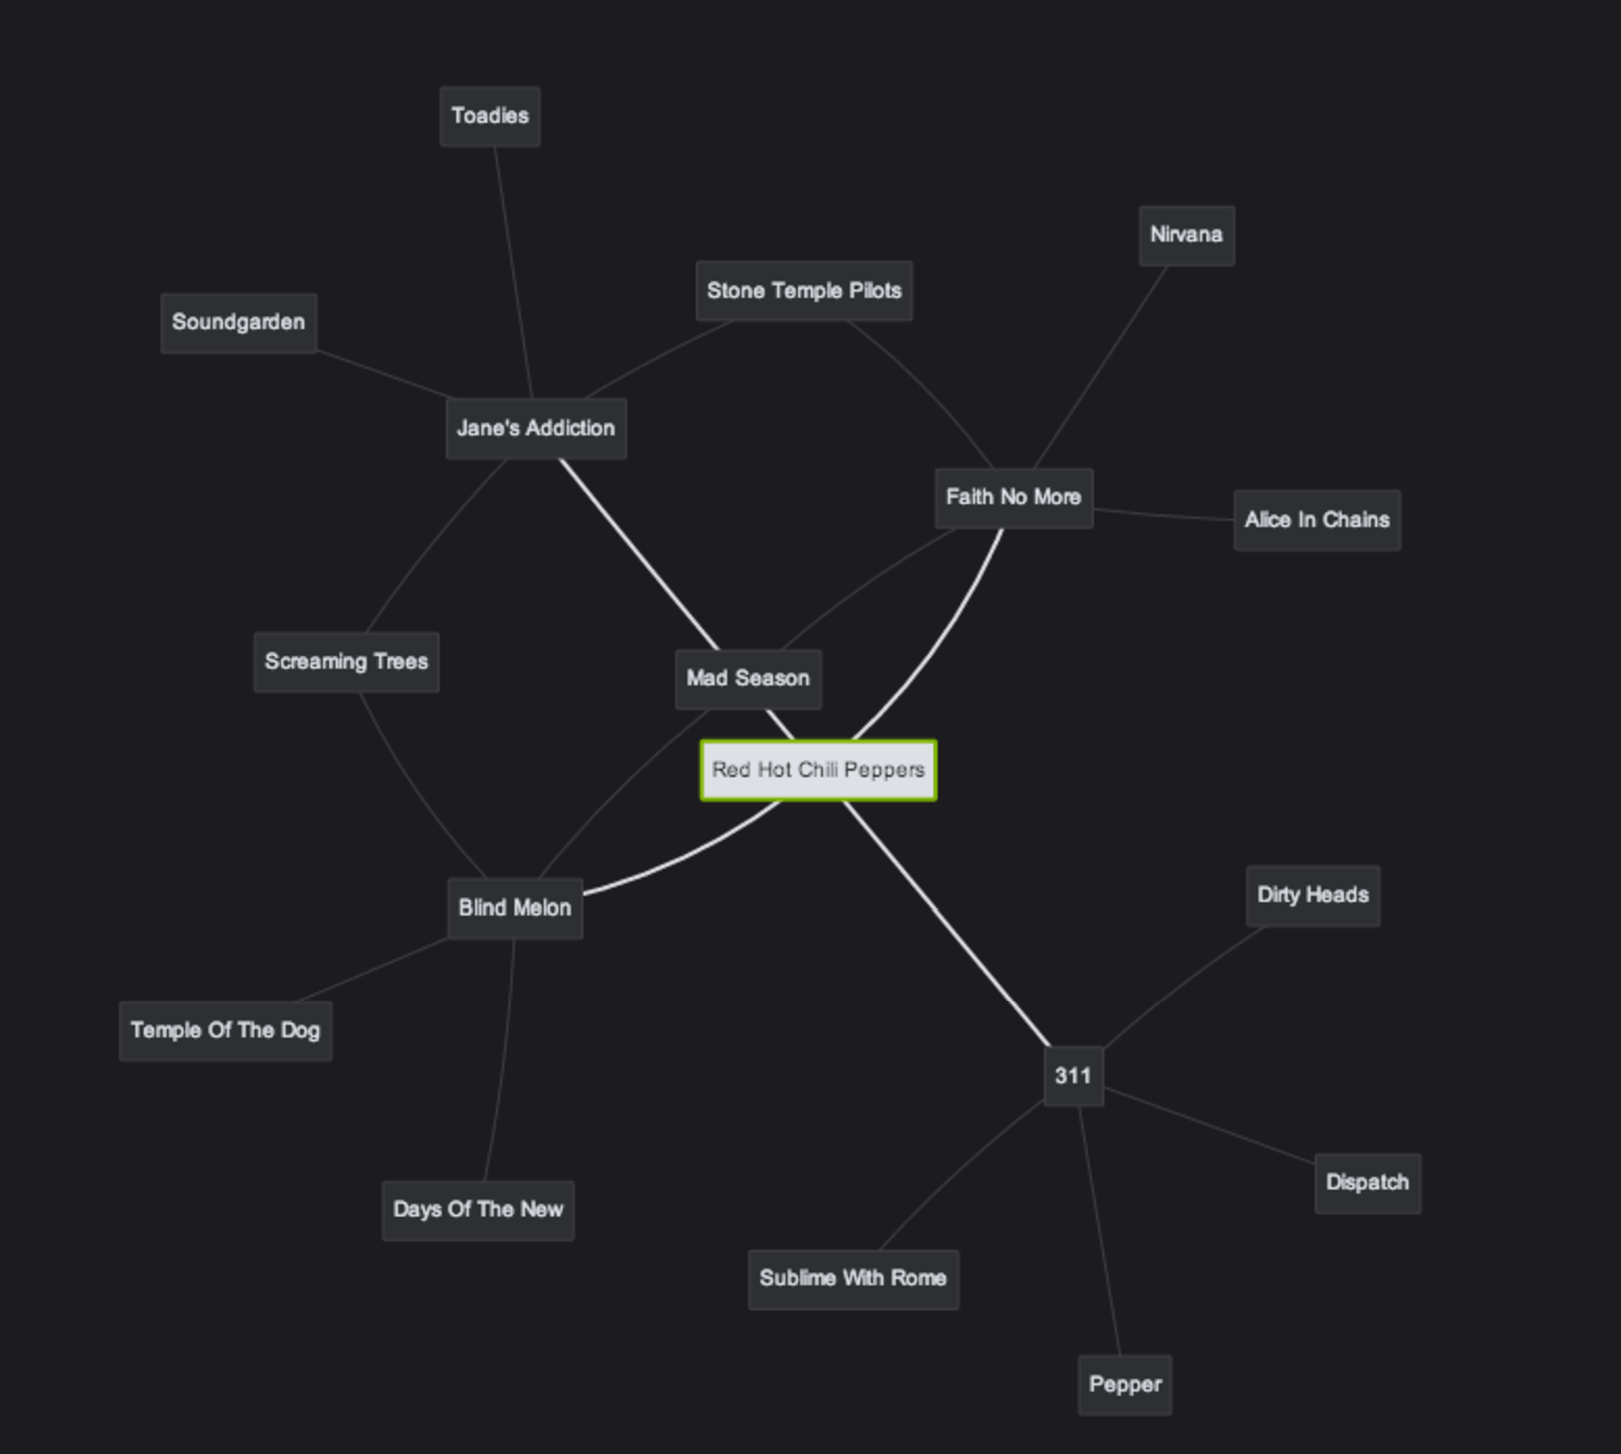
\includegraphics[width=\textwidth]{map_creation_notreemode.pdf}
        \end{center}
        \caption{Graph created with all the connections with "Red Hot Chilli Peppers" as the root node.}
        \label{fig:graph_notreemode}
      \end{figure}

      \hfill \\
      \indent \emph{
      From now on, if the graph is a tree, it will be said that the algorithm is using the \emph{Tree Mode}.
      So the example \ref{fig:graph_treemode} is a \emph{Tree Mode} example, and the examples \ref{fig:graph_notreemode} and \ref{fig:graph_notreemode2} are not \emph{Tree Mode} examples\footnote{
        Note that, sometimes, even if the algorithm is not on tree mode, it might generate a tree, simply because there were no missing edges between the nodes to be added to the graph.
      }.}
      \hfill \\

      Note (\ref{fig:graph_notreemode}) how "Stone Temple Pilots" is now a child of both "Faith No More" and "Jane's Addiction".
      Also note that the same behaviour is visible with the nodes "Mad Season" and "Screaming Trees".

      At this point, the user's perception of the artist "Stone Temple Pilots" is now different from the previous example (Figure~\ref{fig:graph_treemode}).
      These added connections are, in a way, clustering together the most connected nodes.
      In this particular example, one could see an improvement with this approach: it contributes to the user's perception of the artist's network by making sure the user knows that those specific artists are more connected between them, than any others.
      The fact is that only three extra edges where added, meaning there is not much visual clutter in the visualization. \\

      However, that might not always be the case.

      One could argue that the "Mad Season" artist node is already disturbing the visual representation by being drawn over an edge.

      In fact, with the exact same values of branching, depth and tree mode off, when creating a graph for the artist "Mariza", the visual clutter is so strong that the graph becomes confusing and not very helpful: Figure~\ref{fig:graph_notreemode2}.

      \begin{figure}[tb]
        \begin{center}
          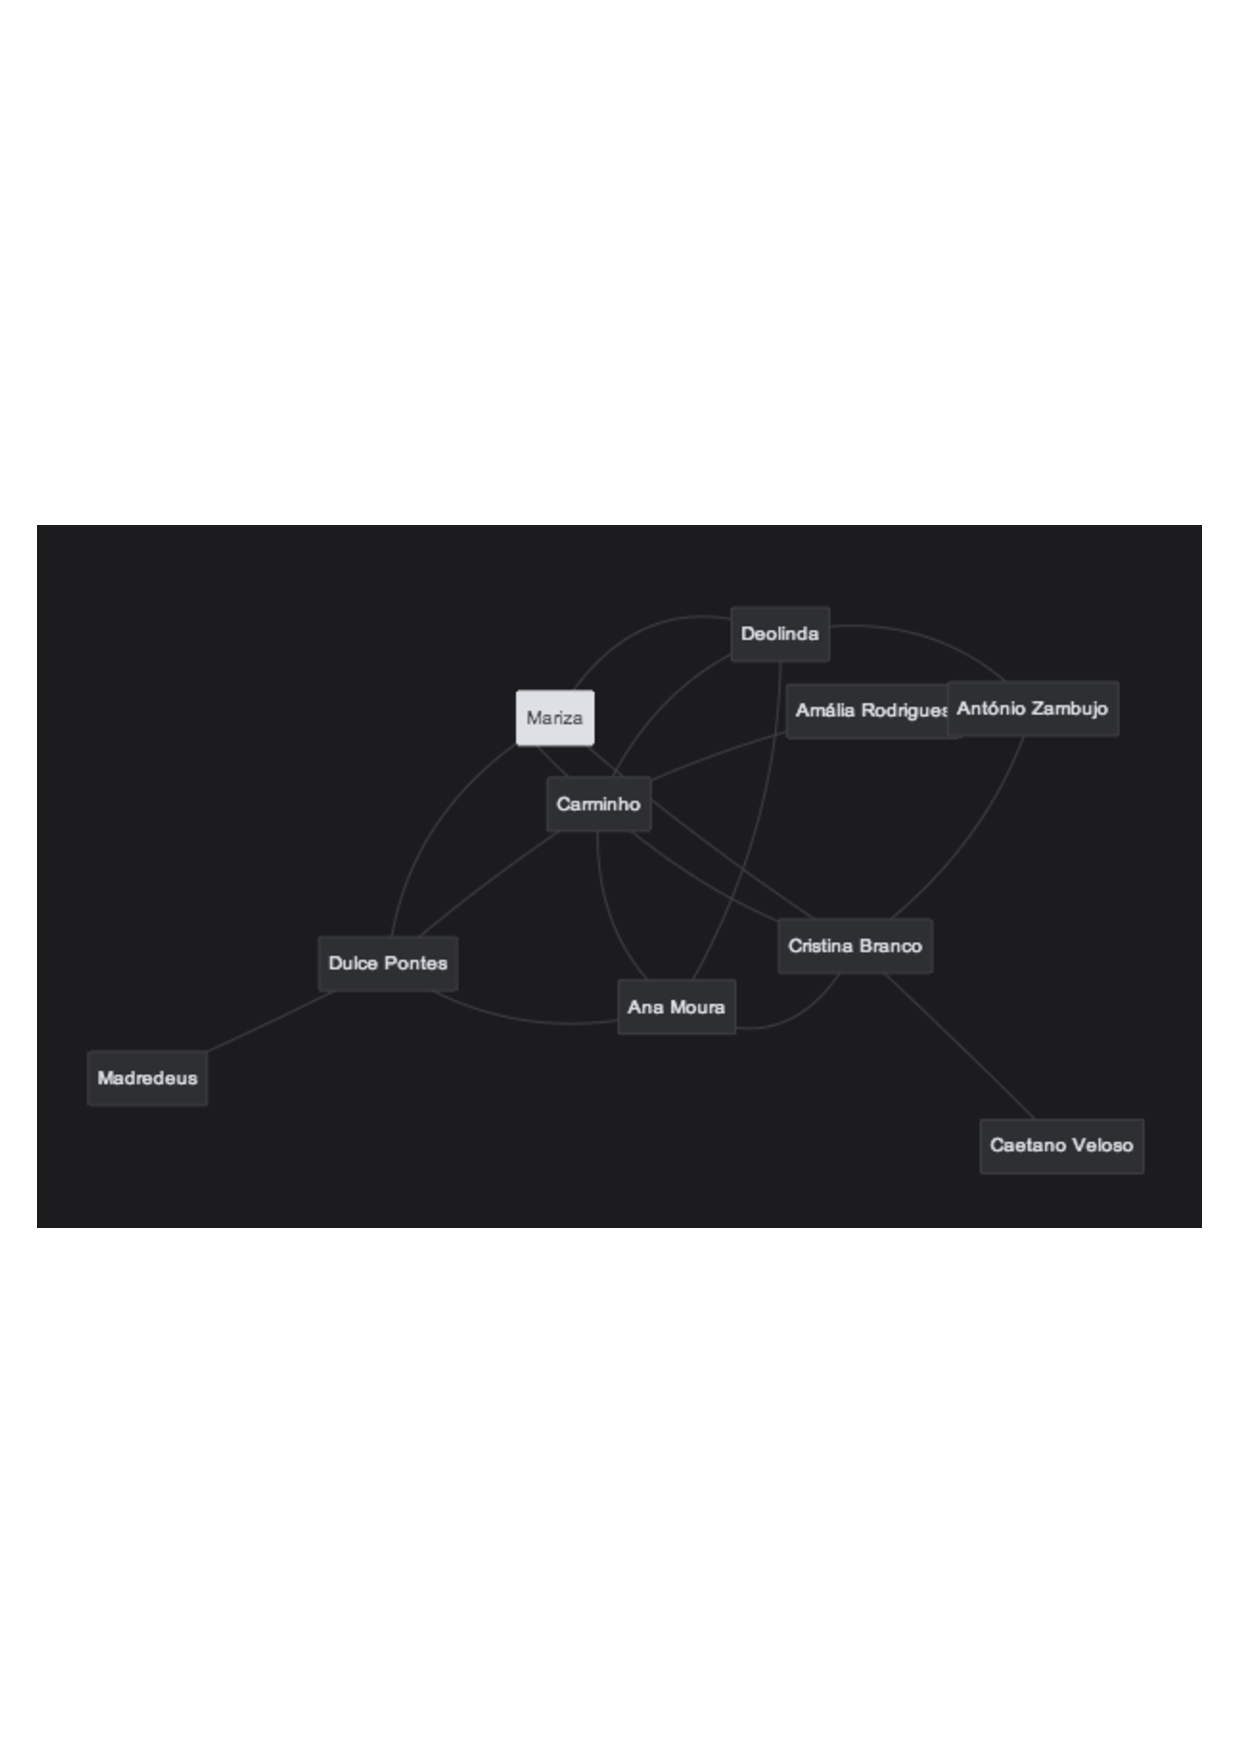
\includegraphics[width=\textwidth]{graph_notreemode2.pdf}
        \end{center}
        \caption{Graph created with all the connections with "Mariza" as the root node.}
        \label{fig:graph_notreemode2}
      \end{figure}

      The cluster of nodes in the center makes it clear that those specific nodes are really connected between them. 
      But then, the edges, that are forcing those nodes together, are creating a visual clutter that might not be so desirable.
      Instead of creating a visual map of the artists' network for the user to perceive, explore and change in its own way, the representation is more contained, static and not so visually appealing.
      \hfill \\

      So on one hand, the \emph{clustering} of the nodes seems like an interesting feature.
      It allows for a much more in-depth user access to the underlining information of the related artists.
      But on the other hand, the focus of the visualization (to show a map of the artists' network) is shifting to this cluster-like representation.

      Both perspectives are advantageous depending on the data they are operating on (as seen in the previous examples).
      So instead of choosing only one method, both were chosen: by default, the graph creation algorithm is on tree mode, and the user can turn it off from a settings menu.
      This allows for the user to choose the visual representation method that suits its needs.

      \paragraph{Depth and Branching values} \hfill \\
      The depth and branching values have been mentioned before in this chapter, but not further explained.

      The \textbf{depth} value of a graph determines how deep the recursive algorithm is.
      The previously presented example (\ref{fig:graph_treemode}) has a depth value of 2.
      The example \ref{fig:graph_depth3} has a depth value of 3.
      \begin{figure}[tb]
        \begin{center}
          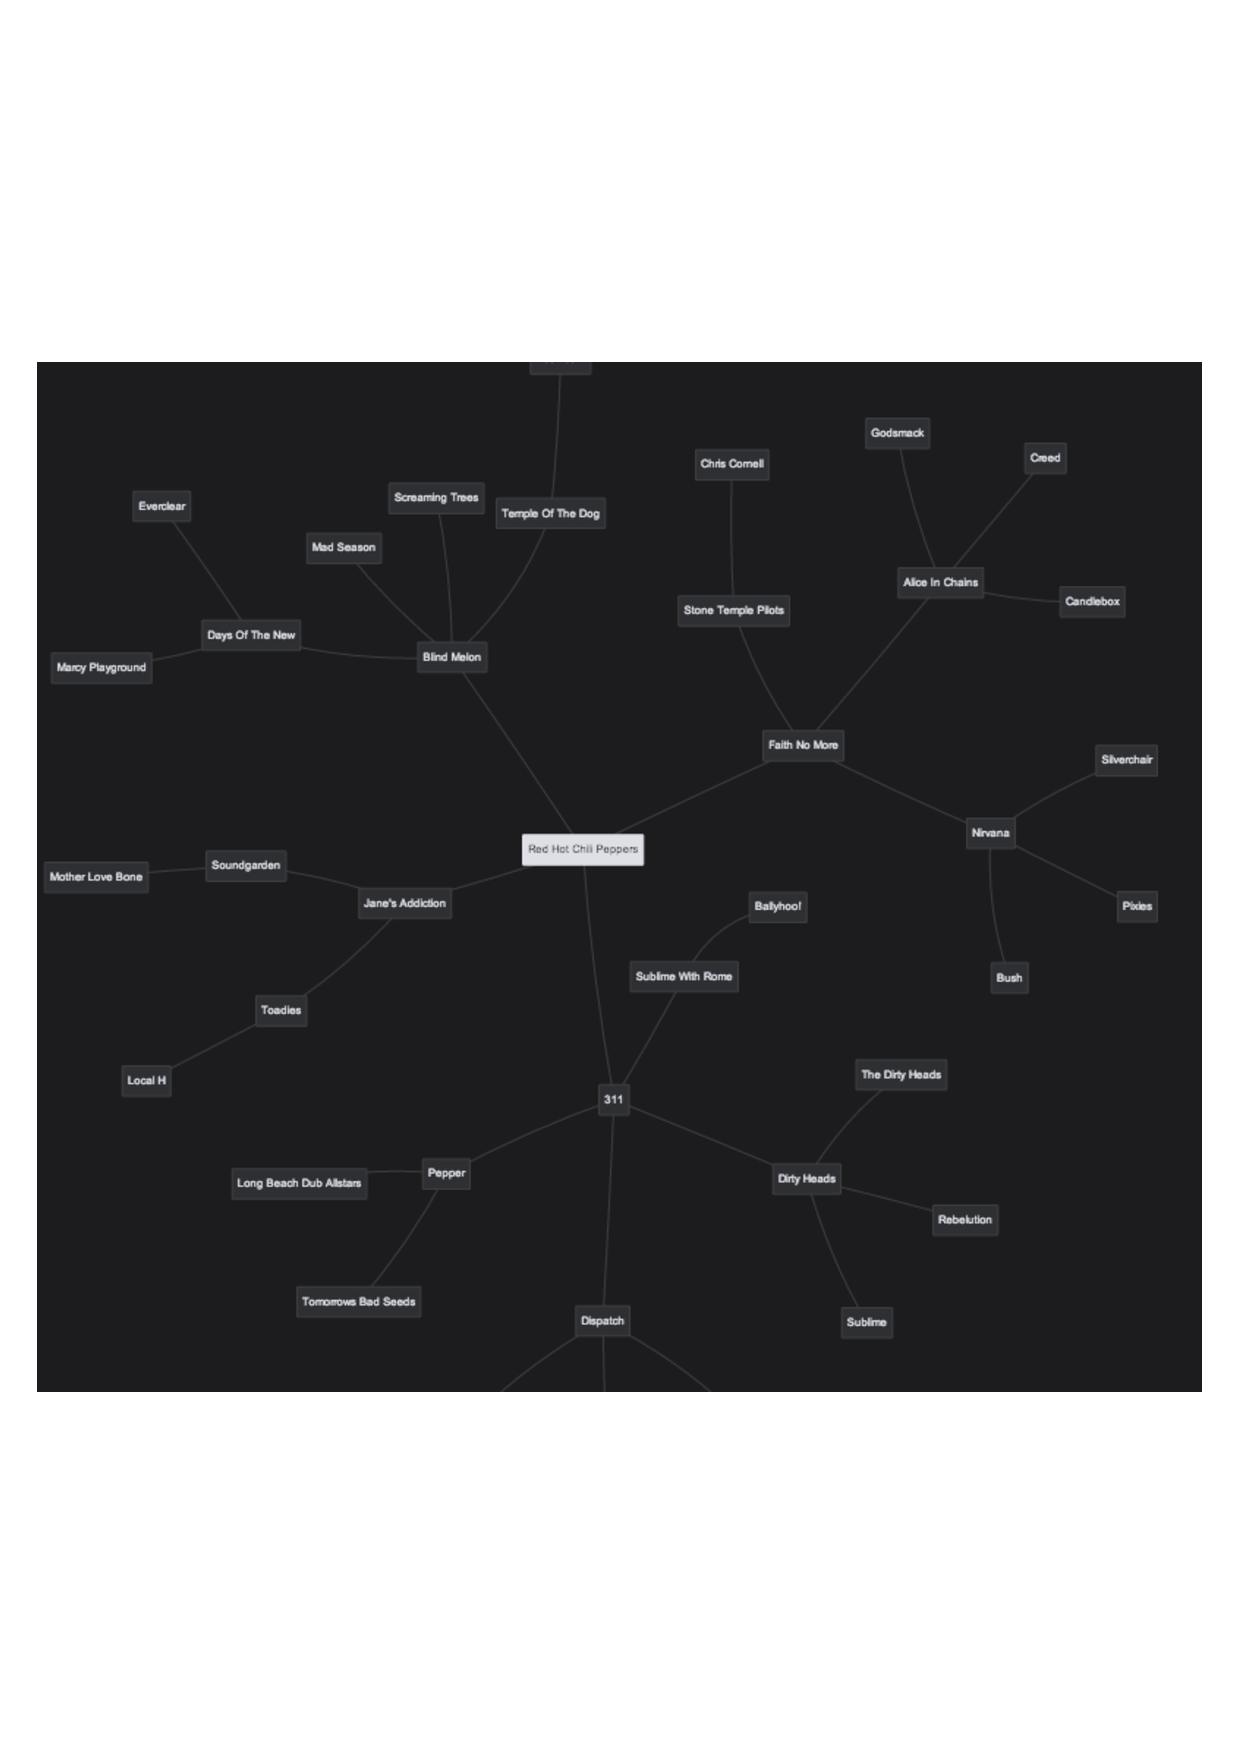
\includegraphics[width=\textwidth]{graph_depth3.pdf}
        \end{center}
        \caption{Graph with depth value of 3}
        \label{fig:graph_depth3}
      \end{figure}
      In short, depth is the maximum distance between the root node and any other node in the graph.

      The \textbf{branching} value of a tree graph determines the maximum number of child nodes a node can have.
      The example \ref{fig:graph_treemode} has 4 branching.

    % subsubsection visualization (end)

    \subsubsection{Visualization Parameters} % (fold)
    \label{ssub:visualization_parameters}
    
    The visualization parameters are the branching and depth values, as well as the option to enable/disable the tree mode.

    To allow the user to change these values, a settings menu was added to the application, and can be seen in Figure~\ref{fig:settings_menu}.
    When the user changes the parameters, the graph refreshes accordingly.

    \begin{figure}
      \begin{center}
        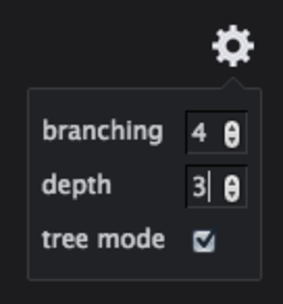
\includegraphics[width=0.8\textwidth]{settings_menu.pdf}
      \end{center}
      \caption{The settings menu that allows the user to change the visualization parameters.}
      \label{fig:settings_menu} 
    \end{figure}

    % subsubsection visualization_parameters (end)

    \subsubsection{Graph Edition} % (fold)
      \label{ssub:edition}

      The available features to edit the graph are as follow: expand node, delete node and create a new map.
      These interactions are available in the Artist Menu (\ref{ssub:artist_info}).

      \paragraph{Expand node} \hfill \\
      This option allows the user to expand a node further (ignoring the graph's branching value).
      Given the previous example \ref{fig:graph_treemode}, if the "Dispatch" node gets expanded, it results in \ref{fig:node_expanded}.

      To put it simply, to expand a node, one performs one iteration of the graph creation algorithm.

      \begin{figure}[tb]
         \begin{center}
           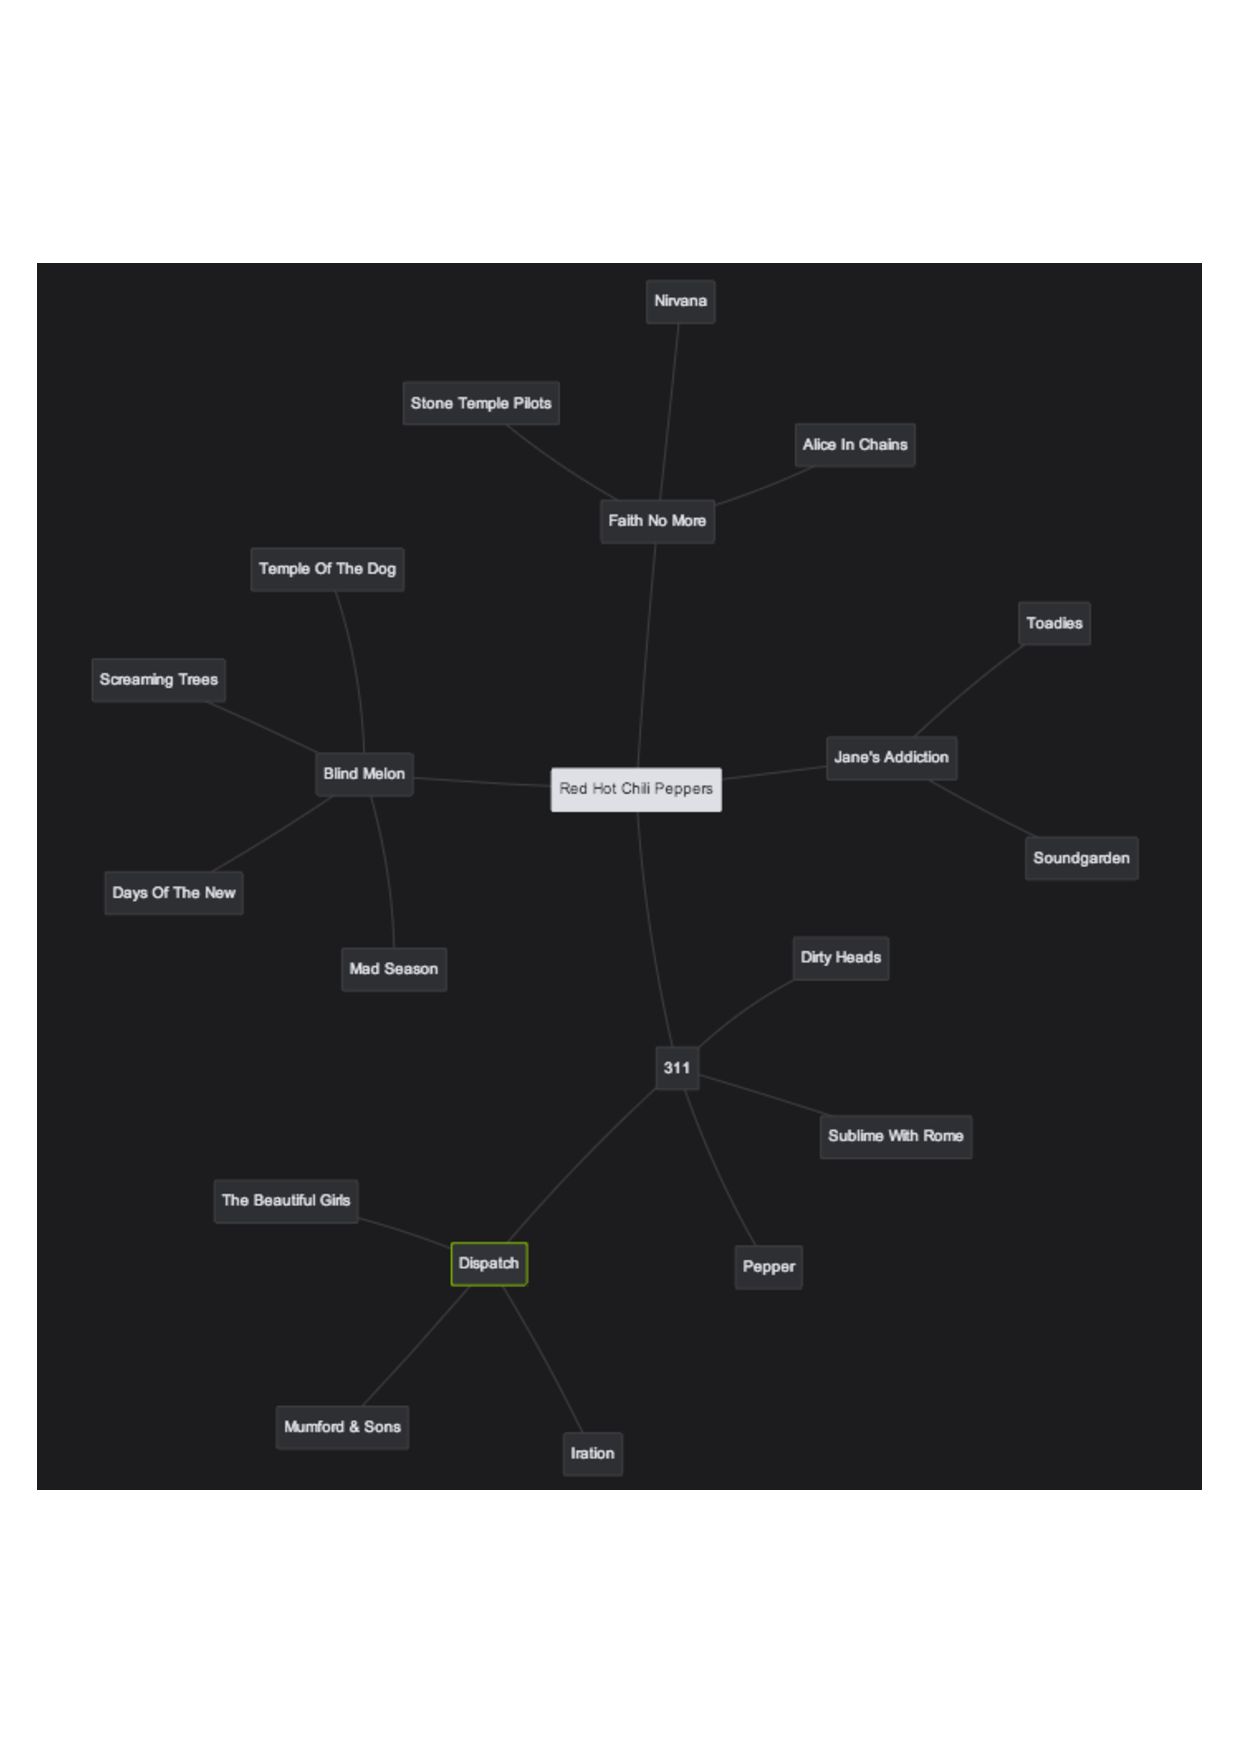
\includegraphics[width=\textwidth]{node_expanded.pdf}
         \end{center}
         \caption{"Dispatch" artist node expanded.}
         \label{fig:node_expanded}
      \end{figure}

      \paragraph{Delete node} \hfill \\
      This options allows the user to delete a node from the graph.
      Useful for when the user wants to construct the graph to its needs.

      \paragraph{New map} \hfill \\
      The user may choose to create a whole new graph from a another node.
      This way the root node will be the selected node.


    % subsubsection edition (end)

    \subsubsection{Artist Info} % (fold)
      \label{ssub:artist_info}
      The user is able to see additional information about artists in the Artist Menu (\ref{fig:artist_menu}) such as its popularity value, albums and tags, as well as perform the \emph{expand} and \emph{new map} functions described in \ref{ssub:edition}.

      \begin{figure}[tb]
        \begin{center}
          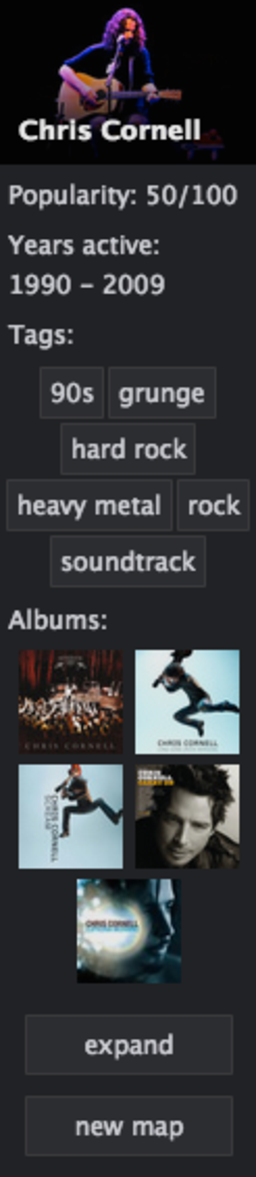
\includegraphics[width=\textwidth]{artist_menu.pdf}
        \end{center}
        \caption{Artist Menu with information about "Chris Cornell"}
        \label{fig:artist_menu}
      \end{figure}

      When the user selects a node by clicking on it, the artist menu updates the displayed information.

      The \emph{popularity} and the \emph{albums} are metadata information retrieved from Spotify's API framework (\ref{ssub:spotify_apps}).
      The tags, however, are not supported by Spotify's API.
      For that, Echonest's API was used.

      \paragraph{Echonest's Terms} \hfill \\
      Echonest's tags are very similar to the most commonly known \emph{music genres} (like jazz, country, rock), but they also might include more alternative descriptive terms (progressive metal, symphonic, soundtrack).

      The connection between the two APIs is possible thanks to the Project Rosetta Stone\footnote{\url{http://developer.echonest.com/docs/v4\#project-rosetta-stone}}.
      For example, to retrieve the terms\footnote{Echonest calls it terms. From now on, terms and tags will be used interchangeably} of an artist from Echonest's metadata API using the Spotify's Artist ID, the following query is used: \\

      \url{
        http://developer.echonest.com/api/v4/artist/terms?api_key=API_KEY&format=json&sort=weight&id=spotify-WW:artist:65nZq8l5VZRG4X445F5kmN
      } \\

      The \emph{id} parameter is similar to the Spotify's URI scheme (\ref{ssub:metadata_api}), and this allows for retrieving extra information about the artist that Spotify's API does not provide.

      \emph{Sort} is another interesting parameter. 
      In general, artists have more than 10 or 15 terms.
      Each term has a value of \emph{frequency} and a value of \emph{weight}, and both are float values that range between zero and one.
      No official documentation was found to explain what do these values represent, but Paul Lamere\footnote{Paul Lamere is Director of Developer Platform at \url{the.echonest.com} (\url{http://the.echonest.com/company}). Also blogs here: \url{http://musicmachinery.com}} explains\footnote{thread in the forum for Echonest's API users - \url{http://developer.echonest.com/forums/thread/353}} that:

      \begin{quote}
      \emph{
        term frequency is directly proportional to how often that term is used to describe that artist
      }
      \end{quote}

      \begin{quote}
      \emph{
        term weight is a measure of how important that term is in describing the artist
      }
      \end{quote}

      So given this, one can conclude that by sorting the terms of an artist by its frequency value, the top terms will be more general (rock, pop, jazz) and not very descriptive or specific of an artist.
      And by sorting the tags by weight, one will get the most descriptive tags of that specific artist.

      Clearly, in this case, for the Artist Menu the weight parameter is very helpful, and so, the sort parameter used for the query is \emph{weight}.
      As seen in \ref{fig:artist_menu}, the tags shown are very descriptive of the artist (grunge, 80s, hard rock). \\

    % subsubsection artist_info (end)

    \subsubsection{Tags Overlay} % (fold)
      \label{ssub:tags_overlay}

      The tags overlay menu (\ref{fig:tags_overlay}) is meant to enhance the user's perception on the displayed artists' nodes regarding their tags.

      \begin{figure}[tb]
        \begin{center}
          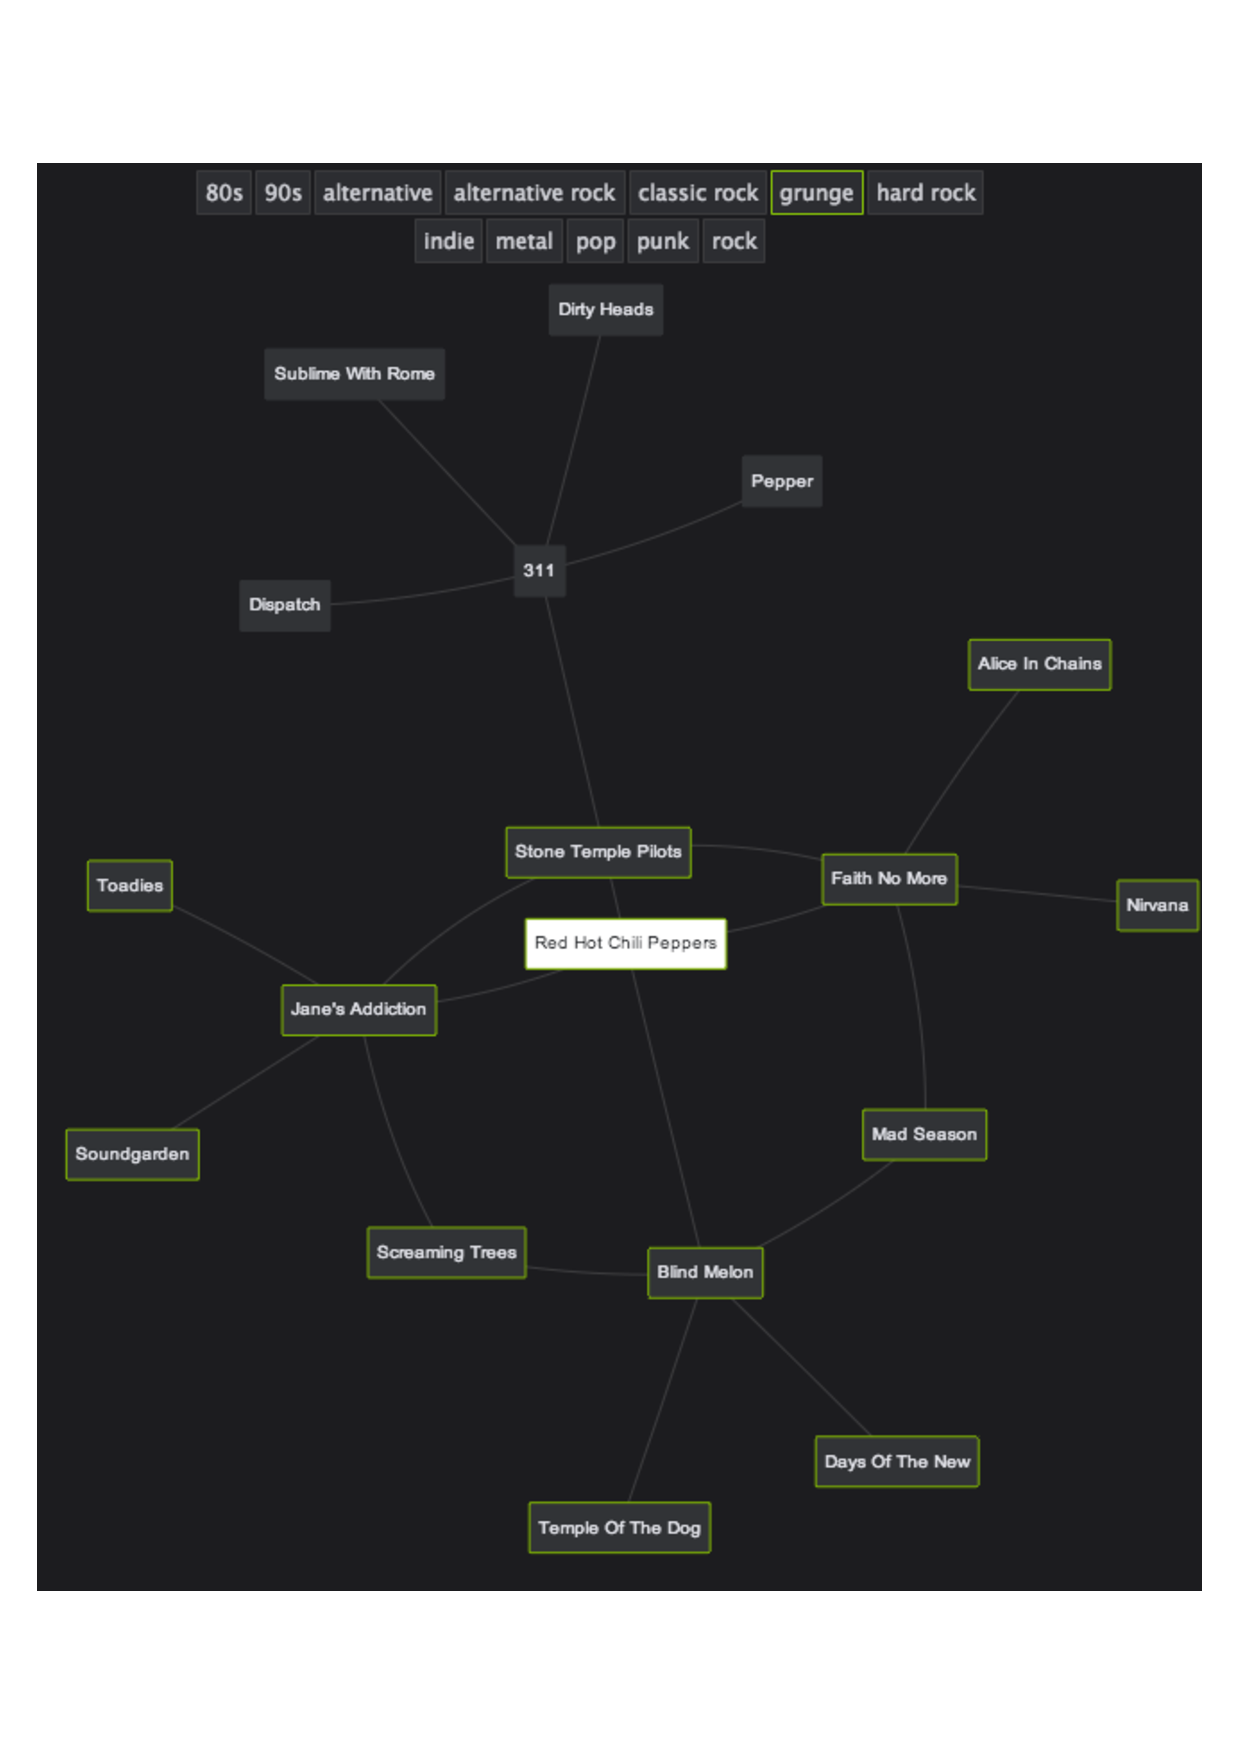
\includegraphics[width=\textwidth]{tags_overlay.pdf}
        \end{center}
        \caption{Tags overlay for the displayed graph. When the tag "grunge" is selected the corresponding artist nodes are selected}
        \label{fig:tags_overlay}
      \end{figure}

      These tags are the same ones used in the Artist Menu (\ref{fig:artist_menu}).

      The tags are selectable, and so, when clicked, the respective artist nodes that are described by those tags, are highlighted (as seen in Figure~\ref{fig:tags_overlay}).

      The tags shown in this menu, are just a small sample of the artists' tags of the whole graph.
      For example, for the graph in the Figure~\ref{fig:graph_anamanaguchi}, the total count of unique tags in the whole graph is 93.
      To select which tags to show, those same 93 tags were sorted by frequency in the graph, and then the top 12 ones are shown.

      This way, the tags in the overlay are significant for the graph, by helping the user to visually group together some related artists.

      \begin{figure}
        \begin{center}
          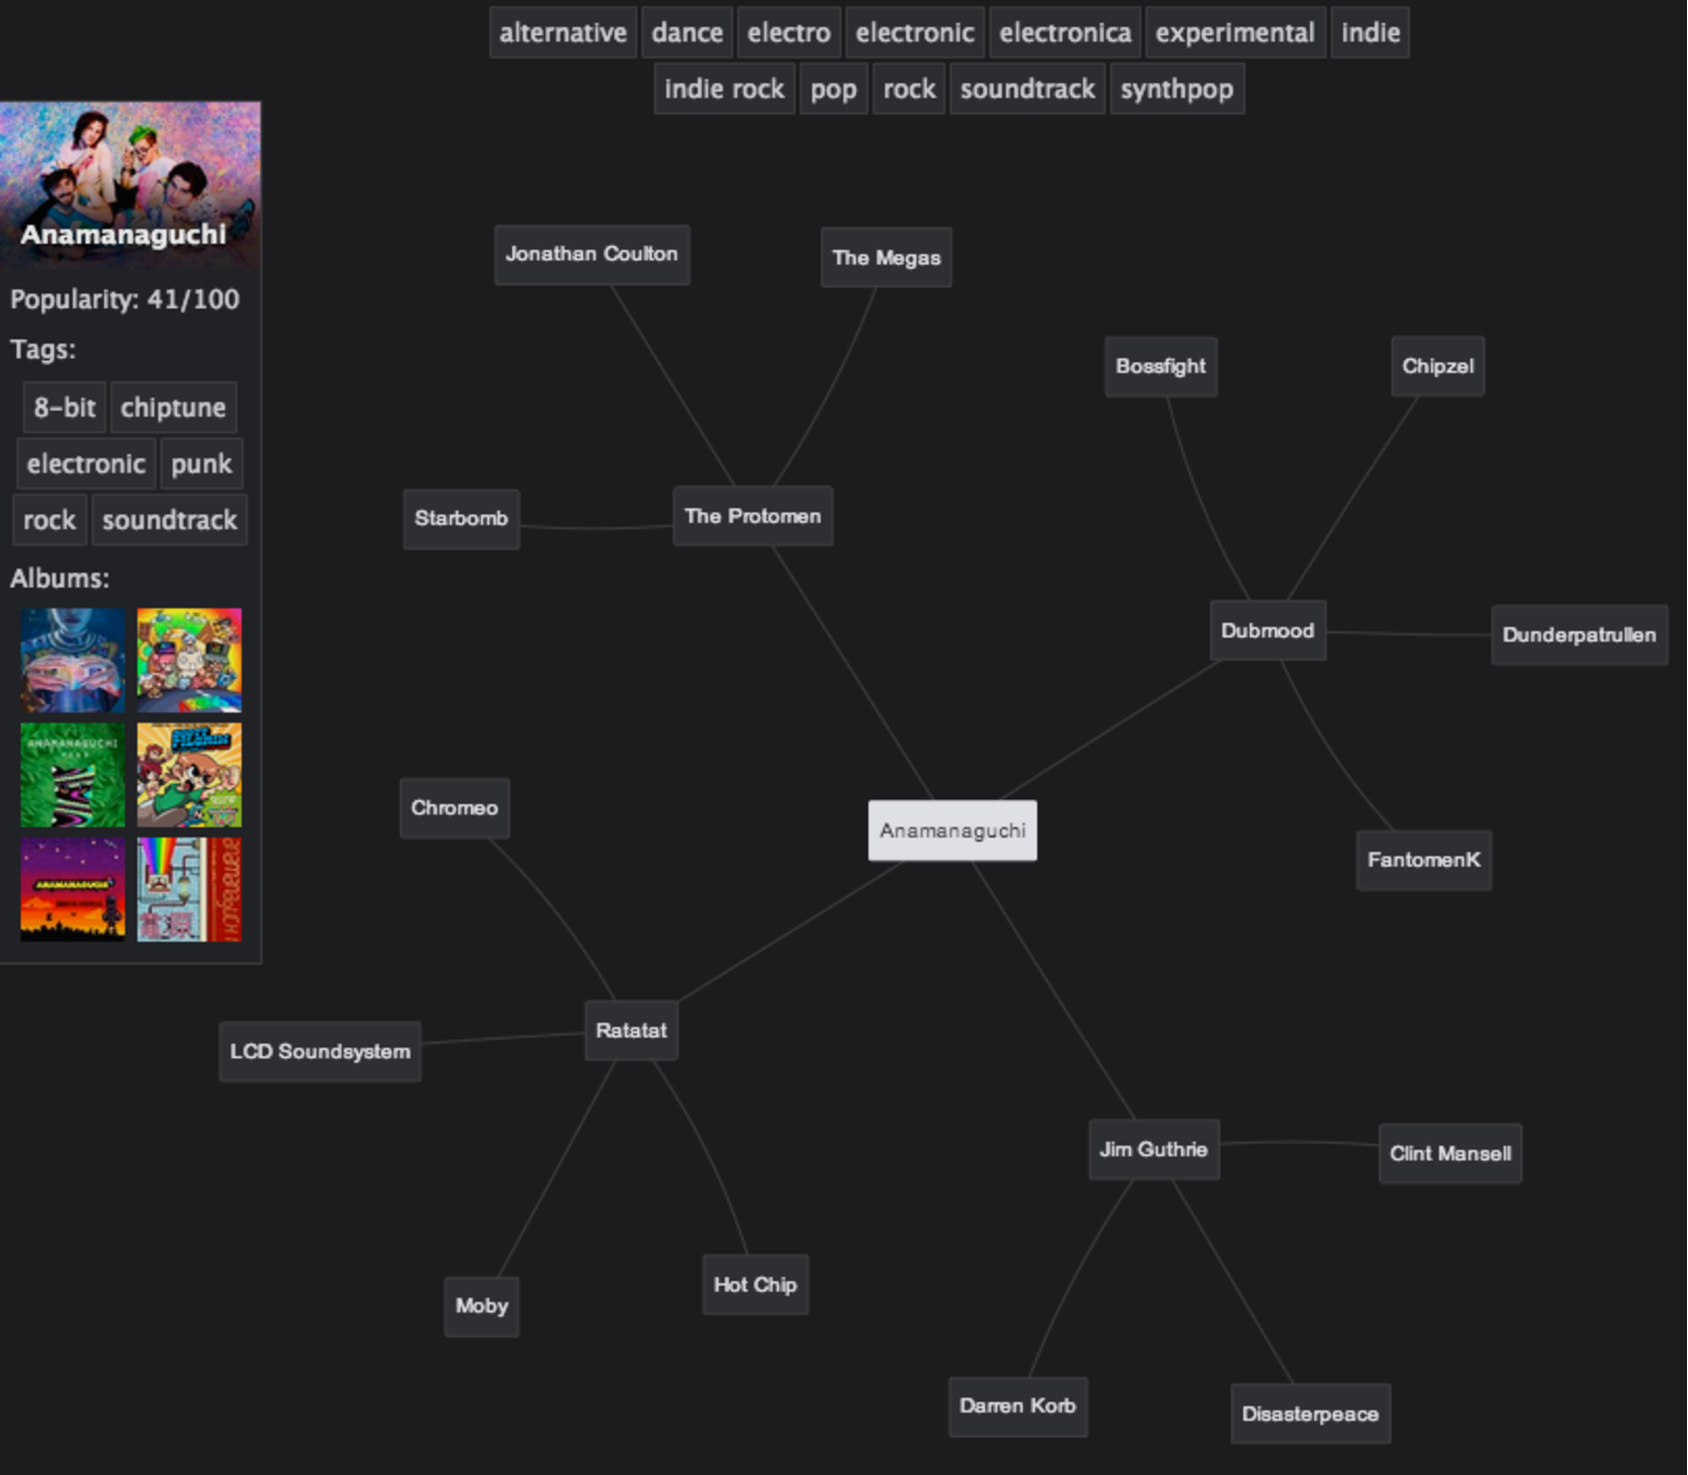
\includegraphics[width=\textwidth]{graph_anamanaguchi.pdf}
        \end{center}
        \caption{Graph for "Anamanaguchi". The tags shown above are only but a small sample of all the tags of all the artists in the graph}
        \label{fig:graph_anamanaguchi}
      \end{figure}

    % subsubsection tags_overlay (end)

  % subsection main_features (end)


  \subsection{Development Processes} % (fold)
    \label{sub:development_process}

    The primal objectives for the RAMA Spotify Application were to implement the basic functionalities that RAMA's website\footnote{\url{http://rama.inescporto.pt/app}} offers.

    Incrementally, they were implemented, tested and added to the application.
    A timeline (chronological order from bottom to top) with the added features (each update release) can be seen in \\ 
    \indent \url{https://github.com/carsy/rama-spotify/releases} \\

    Unit tests were added for each feature.
    The tests were run locally to ensure that nothing broke mean while.
    Also to ensure that every release had the tests passing, the project was integrated in Travis's Continuous Integration\footnote{\url{http://travis-ci.org}} system: \\
    \indent \url{http://travis-ci.org/carsy/rama-spotify}. \\

    This way, after every push of a new release, the project gets build and the unit tests run automatically.

    The solution was also submitted to validation several times during its development.
    After each release, a constant small group of test subjects (3 people) reviewed the state of the application (alfa testers).
    Their feedback would be carried over the next release: bug fixes, improvements, etc.
    This was the testing cycle that allowed to validate the implemented features.
    Given this iterative process of implementation and feedback, the solution would be better prepared for future occasional beta-testing.

    
    % compare with the previous work plan

  % subsection development_processes (end)

% section prototype (end)


\section{Validation} % (fold)
\label{sec:validation}

  In order to validate the proposed method, user tests were done with Spotify users and non-Spotify Users.

  \subsection{User Tests} % (fold)
  \label{sub:user_tests}

    The proposed application is targeted at Spotify Users.
    However, non-Spotify users also tested RAMA's Spotify Application after a few moments of using Spotify's interface.

    During the test, the user was asked to first use Spotify only.
    The task was to find a couple of new artists that the user liked.
    This first task should take no more than 7 minutes.

    Next, the user was asked to open the RAMA application and do the same.
    
    Given this, the user is forced to compare the two approaches: discovering new music with Spotify only, and discovering new music with RAMA's Spotify Application.
  
  % subsection user_tests (end)

  \subsection{Data Analysis} % (fold)
  \label{sub:data_analysis}


  
  % subsection data_analysis (end)
% section validation (end)


\section{Summary} % (fold)


% section summary (end)
%!TEX root = ../report.tex

\chapter{Conclusions}
\label{chap:chap5}

\section*{}


\section{Summary} % (fold)
\label{sec:summary}

  The proposed thesis focused on delivering an enhanced user experience when discovering new music in Spotify's Environment.
  By using RAMA's concept applied in the developed prototype, the user experience when discovering new music as been greatly increased.
  The users felt that RAMA's Spotify Application was natural and intuitive.

  The amount of services that use visual tools for recommending music to users are not that many, although, the ones shown in Chapter~\ref{chap:chap2} are not representative of the whole spectrum.

  Given the overview of the possibilities presented in Chapter~\ref{chap:chap3}, creating a Spotify Application to apply RAMA's concept proved to be the best option to take.

  The proposed modules \ref{intro:obj4} and \ref{item:obj5} were implemented.
  The developed prototype proved to work after the beta-testing results.
  Although, there are a lot of improvements to do, the final result was very appealing to the users.
  All of the beta-testers liked the visual experience and the majority responded positively about using the application in a regular basis to discover new music.

  All of the developed material (code, documentation, wiki, screenshots, demos) can be found in the project's code repository (\url{http://github.com/carsy/rama-spotify}) as well as in the appendix (\ref{appendix}) to this document.

  Two submissions will be sent to the following conferences:
  \begin{itemize}
    \item ISMIR 2014\footnote{\url{http://www.terasoft.com.tw/conf/ismir2014}} - Demo submission\footnote{\url{http://www.terasoft.com.tw/conf/ismir2014/theLBD.html}}
    \item INFORUM 2014\footnote{\url{http://inforum.org.pt/INForum2014}} - Comunication and poster\footnote{\url{http://inforum.org.pt/INForum2014/submissoes}}
  \end{itemize}

% section summary (end)

\section{Discussion} % (fold)
\label{sec:discussion}

  By introducing a visualization tool into a complete service like Spotify, the users felt that their experience with RAMA's application improved their abilities to find new music.
  The tests' results show that RAMA's Spotify Application is a successful approach to music discovery and recommendation.
  Although, the final results point in that direction, after the experiments, 3 beta-testers stated that their music listening habits are not focused on the music artists they are listening to. Instead, they simply pay attention to the songs (mostly, the popular ones), and so, their playlists are track-driven, not artist-driven.
  That might have had presented a problem to those users, since the focus of RAMA is the relations between the artists.
  However, Spotify's API's recommendation system proved to please those users, who started to pay more attention to the name of the artists they listen to.

  Services like Spotify or Rdio, offer a complete set of features that range between playing every track on their catalogue, to saving albums for offline mobile listening.
  With such a vast music catalogue, the user might feel lost and not very motivated to find new music.
  Although these services continue to add features like Spotify's ``Radio''~\cite{spradio}, the user finds it hard to cope with such a large world of available music.

  By introducing this visual aid to music artist's relations, RAMA succeeds in letting the user understand and explore better the whole spectrum of available music.

% section discussion (end)

\section{Future Work} % (fold)
\label{sec:future_work}

  From the developed work so far, a more segmented testing might have been called for, in order to improve the results obtained, as well to better understand the user's needs.

  During the prototype's development and the beta-testing experiments, there were several additional features suggested for RAMA's Spotify Application.
  Most of them were not included in the prototype because of the limited time frame for development, while others seemed to stray from RAMA's focus.
  Nonetheless, every idea is important and might someday contribute to the development of future features for RAMA.

  \paragraph*{Place the action buttons (expand, new map and delete) near the artist node} \hfill \\
  \indent Some users complained that it was hard to notice the action buttons (one user did not even notice them).
  Maybe placing the buttons near the artist node and only show them while hovering it would make more sense.

  \paragraph*{Make it clear that the tags are clickable to the user} \hfill \\
  \indent For some users it was not apparent at first that the upper tags were clickable, they thought it was just an extra information, not something they could interact with.

  \paragraph*{Allow to click-and-hold to preview listening to an artist} \hfill \\
  \indent This Spotify feature could be applied to the nodes so that the user could browse the graph much faster.

  \paragraph*{Select multiple artists or tags} \hfill \\
  \indent Allow the user to select multiple artists (or tags), in order to, for example, generate playlists from that selection.

  \paragraph*{Let the graph update automatically with the current playing artist} \hfill \\
  \indent In order to keep RAMA more alive, the graph would refresh automatically when a new artist starts playing, with the new updated artist as root.
  Maybe an option to keep the graph ``locked'' would allow the user to choose if he/she wants that behaviour or not.

  \paragraph*{Improve artists recommendations} \hfill \\
  \indent The assumption that Spotify's recommendations are valid might not be so desirable.
  Although the results are satisfactory, without knowing the reasons behind those choices of connections, the artists recommendations become inflexible.
  To improve this, one could fully use Echonest's API to fetch the similar artists~\cite{echonestsimilar}.
  The amount of query personalization is much more attractive than Spotify's.

  \paragraph*{Improve the connection between the artists and the tags} \hfill \\
  \indent As an improvement of the previous idea, the connections between the artists and the overlaying tags could become more related, and so, the intersection of tags between artists could be used to improve the recommendations (creation of connections). 

  \paragraph*{Include an alternate view with tags as nodes, instead of artists} \hfill \\
  \indent Some users suggested that the tags overlay was an interesting point of view, and so, if the graph could be drawn using the tags instead, the resulting map would then be an alternative view of the application.

  \paragraph*{Improve artists recommendations with Social Networks' data} \hfill \\
  \indent A user suggested that the connections between the artist nodes could be improved using information from social networks.
  Spotify already has the possibility for the user to integrate his/her Facebook\footnote{\url{http://facebook.com}} account, and so, this information could be used to personalize the recommendations \cite{Fields2011}.

  \paragraph*{Cluster groups of artists} \hfill \\
  \indent Cluster groups of artists to create a geographical representation of what the entire network of available artists could be like.

  \paragraph*{Tag mind map} \hfill \\
  \indent In a way to try and complement the two previous ideas, a clustering of the tags would create an interesting mind map of the current genres.
  And since there are indeed music genres that are similar (for example, metal and celtic metal) the map would be browsable.

  \paragraph*{Information} \hfill \\
  \indent Add an information UI component to help the users understand better the visualization parameters (a tutorial-like component) - although those parameters are advanced settings (not strictly necessary for the user to interact with) it might be a good idea to give more power to the user and make these settings easy to understand.

  \paragraph*{3D Visualization} \hfill \\
  \indent Regarding the discussion in \ref{ssub:visualization}, if the graph is not a tree, the visual clutter can degradate the user's experience.
  Some users suggested a 3D Visualization for these cases.
  This approach can be in fact be a good solution to the problem \cite{Lamere2007using3D}.

  \paragraph*{Show more tags} \hfill \\
  \indent The list of tags shown in the Tags overlay is trimmed as mentioned in \ref{ssub:tags_overlay}, but sometimes the user might want to see more tags.
  A possibility to solve this problem could be to make the list scrollable or to add a "show more" button.

  \paragraph*{Improve the visualization of the connections} \hfill \\
  \indent The length of the edges of the graph could have a repulsion value inversely proportional to how strong the connection between the artists are.
  This might help the user to discover new music quicker than before.



% section future_work (end) 

%%----------------------------------------
%% Final materials
%%----------------------------------------

%% Bibliography
%% Comment the next command if BibTeX file not used
%% bibliography is in ``myrefs.bib''
\PrintBib{myrefs}

%% comment next 2 commands if numbered appendices are not used
\appendix
\chapter{Loren Ipsum} \label{ap1:loren}

Depois das conclusões e antes das referências bibliográficas,
apresenta-se neste anexo numerado o texto usado para preencher a
dissertação.

\section{O que é o \emph{Loren Ipsum}?}

\emph{\textbf{Lorem Ipsum}} is simply dummy text of the printing and
typesetting industry. Lorem Ipsum has been the industry's standard
dummy text ever since the 1500s, when an unknown printer took a galley
of type and scrambled it to make a type specimen book. It has survived
not only five centuries, but also the leap into electronic
typesetting, remaining essentially unchanged. It was popularised in
the 1960s with the release of Letraset sheets containing Lorem Ipsum
passages, and more recently with desktop publishing software like
Aldus PageMaker including versions of Lorem Ipsum. 

\section{De onde Vem o Loren?}

Contrary to popular belief, Lorem Ipsum is not simply random text. It
has roots in a piece of classical Latin literature from 45 BC, making
it over 2000 years old. Richard McClintock, a Latin professor at
Hampden-Sydney College in Virginia, looked up one of the more obscure
Latin words, consectetur, from a Lorem Ipsum passage, and going
through the cites of the word in classical literature, discovered the
undoubtable source. Lorem Ipsum comes from sections 1.10.32 and
1.10.33 of ``de Finibus Bonorum et Malorum'' (The Extremes of Good and
Evil) by Cicero, written in 45 BC. This book is a treatise on the
theory of ethics, very popular during the Renaissance. The first line
of Lorem Ipsum, ``Lorem ipsum dolor sit amet\ldots'', comes from a line in
section 1.10.32.

The standard chunk of Lorem Ipsum used since the 1500s is reproduced
below for those interested. Sections 1.10.32 and 1.10.33 from ``de
Finibus Bonorum et Malorum'' by Cicero are also reproduced in their
exact original form, accompanied by English versions from the 1914
translation by H. Rackham.

\section{Porque se usa o Loren?}

It is a long established fact that a reader will be distracted by the
readable content of a page when looking at its layout. The point of
using Lorem Ipsum is that it has a more-or-less normal distribution of
letters, as opposed to using ``Content here, content here'', making it
look like readable English. Many desktop publishing packages and web
page editors now use Lorem Ipsum as their default model text, and a
search for ``lorem ipsum'' will uncover many web sites still in their
infancy. Various versions have evolved over the years, sometimes by
accident, sometimes on purpose (injected humour and the like). 

\section{Onde se Podem Encontrar Exemplos?}

There are many variations of passages of Lorem Ipsum available, but
the majority have suffered alteration in some form, by injected
humour, or randomised words which don't look even slightly
believable. If you are going to use a passage of Lorem Ipsum, you need
to be sure there isn't anything embarrassing hidden in the middle of
text. All the Lorem Ipsum generators on the Internet tend to repeat
predefined chunks as necessary, making this the first true generator
on the Internet. It uses a dictionary of over 200 Latin words,
combined with a handful of model sentence structures, to generate
Lorem Ipsum which looks reasonable. The generated Lorem Ipsum is
therefore always free from repetition, injected humour, or
non-characteristic words etc. 


%% Index
%% Uncomment next command if index is required
%% don't forget to run ``makeindex mieic-en'' command
%\PrintIndex

\end{document}
